\documentclass[a4paper,11pt]{book}
\usepackage{pgfplots}
\usepackage{float}
\usepackage[T1]{fontenc}
\usepackage[utf8]{inputenc}
\usepackage{lmodern}
%%%%%%%%%%%%%%%%%%%%%%%%%%%%%%%%%%%%%%%%%%%%%%%%%%%%%%%%%
% Source: http://en.wikibooks.org/wiki/LaTeX/Hyperlinks %
%%%%%%%%%%%%%%%%%%%%%%%%%%%%%%%%%%%%%%%%%%%%%%%%%%%%%%%%%
\usepackage{hyperref}
\usepackage{graphicx}

\usepackage[spanish, es-tabla]{babel}
\usepackage{amsmath}
\usepackage{amsfonts}
\usepackage{amssymb}
%%%%%%%%%%%%%%%%%%%%%%%%%%%%%%%%%%%%%%%%%%%%%%%%%%%%%%%%%%%%%%%%%%%%%%%%%%%%%%%%
% 'dedication' environment: To add a dedication subsubsection at the start of book %
% Source: http://www.tug.org/pipermail/texhax/2010-June/015184.html            %
%%%%%%%%%%%%%%%%%%%%%%%%%%%%%%%%%%%%%%%%%%%%%%%%%%%%%%%%%%%%%%%%%%%%%%%%%%%%%%%%
\newenvironment{dedication}
{
   \cleardoublepage
   \thispagestyle{empty}
   \vspace*{\stretch{1}}
   \hfill\begin{minipage}[t]{0.66\textwidth}
   \raggedright
}
{
   \end{minipage}
   \vspace*{\stretch{3}}
   \clearpage
}



\begin{document}

	\begin{center}
		\vspace*{-1in}
%		\begin{figure}[htb]
%		\begin{center}
%		\includegraphics[width=8cm]{./figuras/logo}
%		\end{center}
%		\end{figure}

		\textbf{{\normalsize UNIVERSIDAD AUTÓNOMA DEL ESTADO DE HIDALGO}}\\
		\vspace*{0.03in}
		{{\small \textbf{INSTITUTO DE CIENCIAS BÁSICAS E INGENIERÍA}}} \\
		\vspace*{0.03in}
		{\textbf{{\footnotesize LICENCIATURA EN SISTEMAS COMPUTACIONALES}} }\\
		
	
\vspace*{1in}
\begin{Large}
{\textbf{{\Huge PROYECTO FINAL}}} \\
\end{Large}
\begin{Large}
\textbf{{\LARGE MINERÍA DE DATOS}} \\
\end{Large}
\vspace*{1in}



\vspace*{0.1in}


\vspace*{0.3in}
\rule{80mm}{0.1mm}\\
\vspace*{0.1in}

\begin{Large}
Alumno: \\
David Zahid Jiménez Grez. \\
\end{Large}
\begin{Large}
Asesor: \\
Dra. Anilú Franco Arcega. \\
\end{Large}
\vspace*{0.8in}
\begin{Large}
Fecha: 26 de Mayo de 2014
\end{Large}
\end{center}







%%%%%%%%%%%%%%%%%%%%%%%%%%%%%%%%%%%%%%%%%%%%%%%%%%%%%%%%%%%%%%%
% Add a dedication subsubsection to dedicate your book to someone %
%%%%%%%%%%%%%%%%%%%%%%%%%%%%%%%%%%%%%%%%%%%%%%%%%%%%%%%%%%%%%%%
%\begin{dedication}
%Dedicado a mi.
%\end{dedication}

%%%%%%%%%%%%%%%%%%%%%%%%%%%%%%%%%%%%%%%%%%%%%%%%%%%%%%%%%%%%%%%%%%%%%%%%
% Auto-generated table of contents, list of figures and list of tables %
%%%%%%%%%%%%%%%%%%%%%%%%%%%%%%%%%%%%%%%%%%%%%%%%%%%%%%%%%%%%%%%%%%%%%%%%




\tableofcontents

\listoffigures
\listoftables

\mainmatter

%%%%%%%%%%%
% Resumen %
%%%%%%%%%%%
\section*{{\Huge Resumen}}
\addcontentsline{toc}{section}{\protect\numberline{}Resumen}%
Este proyecto en primer lugar describe los métodos de clasificación supervisada utilizados, así como la descripción de la plataforma de software para minería de datos conocida como Weka, la cual se utilizó para el procesamiento de los conjuntos de datos. \\\\
A continuación expone cada uno de los conjuntos de datos utilizados, así como las instancias y atributos con las que éstos cuentan, cabe mencionar que los métodos de clasificación supervisada utilizados fueron (Naïve Bayes, Árboles de Decisión, Redes Neuronales, K-Vecinos y Máquinas de Vectores de Soporte.), además, aludir que para la evaluación se utilizó la forma cross-validation (Validación Cruzada). Aunado a esto, por medio de gráficas se muestran los resultados de los métodos de clasificación supervisada, y en éstas se observa el porcentaje de clasificación y tiempo de cada uno de éstos. \\\\
Seguidamente, por cada conjunto de datos que se analizó, se concluye cuál de los métodos obtiene el mejor resultado, tomando en cuenta el mejor porcentaje de clasificación correcta y el que logró el menor tiempo de procesamiento. \\\\
Finalmente, este documento presenta la conclusión de todo el trabajo y una conclusión general del análisis de los conjuntos de datos.
%%%%%%%%%%%%%%%%%%%%%
%Sección del Resumen%
%%%%%%%%%%%%%%%%%%%%%


%%%%%%%%%%%%
%ESPACIO   %
%%%%%%%%%%%%
\cleardoublepage %Salto para dos páginas
%%%%%%%%%%%%%%%%%%
%FINALIZA ESPACIO%
%%%%%%%%%%%%%%%%%%
%%%%%%%%%%%%
% Abstract %
%%%%%%%%%%%%


\section*{{\Huge Abstract}}
\addcontentsline{toc}{section}{\protect\numberline{}Abstract}%
%%%%%%%%%%%%%%%%%%%%%%
%Sección del Abstract%
%%%%%%%%%%%%%%%%%%%%%%
This project in first place describes supervised classification methods used as well as the description of the software platform for data mining known as Weka, which was used to process data sets. \\\\
Then exposes each of the used data sets and the instances and attributes with which they have, we should mention that the supervised classification methods used were (Naïve Bayes, Decision Trees, Neural Networks, K-Neighbours and Machines Support Vector.) also allude that the cross-validation assessment form was used. Added to this, by means of graphics supervised classification methods results are shown, and the percentage of these classification and each time they are observed. \\\\
Followed, for each data set analyzed, we conclude which method gets the best result, taking into account the best percentage of correct classification and which has the lowest processing time. \\\\
Finally, this paper presents the conclusion of all work and a general conclusion of the analysis of data sets.
%%%%%%%%%%%%
%ESPACIO   %
%%%%%%%%%%%%
\cleardoublepage %Salto para dos páginas
%%%%%%%%%%%%%%%%%%
%FINALIZA ESPACIO%
%%%%%%%%%%%%%%%%%%
%%%%%%%%%%%%%%%%
% Introducción %
%%%%%%%%%%%%%%%%
\section*{{\Huge Introducción}}
\addcontentsline{toc}{section}{\protect\numberline{}Instrucción}%
%%%%%%%%%%%%%%%%%%%%%%%%%%
%Sección del Introducción%
%%%%%%%%%%%%%%%%%%%%%%%%%%


%%%%%%%%%%%%%%%%%%%%
% Minería de Datos %
%%%%%%%%%%%%%%%%%%%%



%%%%%%%%%%%%%%%%%%%%%%%%%%%%%%
%Sección de Minería de Datos%
%%%%%%%%%%%%%%%%%%%%%%%%%%%%%%

La minería de datos es un conjunto de técnicas que nos ayudan a explorar información valiosa de un conjunto de datos con el fin de extraer información útil para la toma de decisiones. 
La minería de datos principalmente se usa para describir y predecir; Existen dos modelos que son utilizados dentro de la minería de datos, el modelo descriptivo y el predictivo.
La minería de datos puede utilizarse en distintas áreas, algunas de las aplicaciones en general donde se presta la minería de datos son:
\begin{itemize}
\item Aplicaciones financieras y banca.
\item Aplicaciones de mercado, distribución y comercio.
\item Aplicaciones de seguro y salud privada.
\item Aplicaciones  de educación.
\item Aplicaciones en procesos industriales.
\item Aplicaciones en medicina.
\item Aplicaciones en biología, bioingeniería.
\end{itemize}
La minería de datos es una disciplina que abarca muchos aspectos de nuestra vida real.
\\
Modelo descriptivo:
\begin{itemize}
\item Agrupación.
\end{itemize}
Modelo preventivo:
\begin{itemize}
\item Clasificación.
\item Regresión.
\end{itemize}

%%%%%%%%%%%%%%%%%%%%%%%%%%%%%
% Clasificación Supervisada %
%%%%%%%%%%%%%%%%%%%%%%%%%%%%%
%%%%%%%%%%%%%%%%%%%%%%%%%%%%%%%%%%%%%%
%Sección de Clasificación Supervisada%
%%%%%%%%%%%%%%%%%%%%%%%%%%%%%%%%%%%%%%

%CORREGIR EN OTRO MOMENTO%
En este tipo de clasificación se tiene un conjunto de ejemplos, los
cuales tienen asociados un atributo llamado la clase de cada ejemplo, tendremos entonces
algún mecanismo de entrenamiento en base a este conjunto, para permitirnos distinguir las
clases sobre ejemplos de prueba que proporcionemos.
%%%%%%%%%%%%%%%%%%%%%%%%%%%%%
% Objetivo del trabajo %
%%%%%%%%%%%%%%%%%%%%%%%%%%%%%

%%%%%%%%%%%%%%%%%%%%%%%%%%%%%%%%%%
%Sección del Objetivo del trabajo%
%%%%%%%%%%%%%%%%%%%%%%%%%%%%%%%%%%
Este trabajo se realizo para la observación de la eficiencia de los métodos, tanto en tiempo como en calidad de clasificación, en cada conjunto de entrenamiento.

%%%%%%%%%%%%%%
% Capítulo 1 %
%%%%%%%%%%%%%%
\chapter{Algoritmos de Minería de Datos}
%%%%%%%%%%%%%%%%%%%%%%%%%%
%Sección del capítulo 1%
%%%%%%%%%%%%%%%%%%%%%%%%%%
Uno de los aspectos más relevantes de la minería de datos es la clasificación de objetos, un objeto en este experimento puede ser tomado como una instancia dentro de un conjunto de datos que representa el conjunto de entrenamiento. Existen diversas métodos para clasificar este objeto, en este capítulo se describen breve mente los métodos utilizados en Weka para procesar los conjunto de datos, entre ellos podemos mencionar el método Naïve Bayes que es aquel que nos permite clasificar un objeto dependiendo con base en sus atributos discretos o continuos para los cuales utiliza formulas diferentes, también está el método de árboles que clasifica un objeto con base en el árbol de decisión que construye y éste va evaluando cada atributo y descartando los que no entran dentro de sus ramas.
Un método muy utilizado en la inteligencia artificial es el de Perceptron Simple que en general arroja muy buenos resultado pero resulta más difícil de interpretar en la minería de datos. 
Otro método que resulta bastante interesante y que fue de los primeros en desarrollarse es K-vecinos este método calcula la distancia de un objeto a otro y clasifica dicho objeto dentro de la clase de aquellos a los que más se parece o con quienes tiene menor distancia.  El método de Máquinas de Vectores de Soporte es otro de los método utilizados este método crea hiperplanos como fronteras de decisión \cite{Datamining} .

\section{Método Naïve Bayes (NB)}

El método bayesiano es uno de los más utilizados,  se utiliza cuando se tiene incertidumbre o se requiere verificar  si un objeto pertenece o no a una clase, ya que permite calcular la probabilidad asociada a dicha hipótesis, dentro del método \textbf{NB}  se dice que todos los atributos son independientes, conocido el valor de la clase, en este teorema se establece que no importan los atributos que tengo, aun así son válidos para cada una de las clases que se tiene,  se establece: "la probabilidad de que un atributo pertenezca a una clase, por la probabilidad de cada atributo, dadas, dados los valores de cada atributo,  ej. Si el máximo pertenece a esa  clase, es precisamente esa clase la que se devuelve". 
Si el atributo es discreto la probabilidad se obtiene por estimación de máxima verosimilitud\cite{Datamining}.

\begin{equation} \label{eq:Equación 1}
\frac{P(X_i| pa(X_i))}{n(X_i| pa(X_i))}
= \frac{n(X_i,Pa(X_i))}{
n(Pa(X_i))
}
\end{equation}
Estimación basada en la Ley de Sucesión de LaPlace.
\begin{equation} \label{eq:Estimación basada en la Ley de Sucesión de LaPlace.}
P(X_i| pa(X_i))
= \frac{n(X_i,Pa(X_i))+1}{
n(Pa(X_i))+|\Omega(X_i)|
}
\end{equation}
La cardinalidad es el número de posibles valores que puede tener el atributo evaluado.
Si X es continuo el atributo sigue una distribucion normal calcula la media y la desviacion
estandar.
\begin{equation}
P(X_i| c)\alpha N(\mu,\sigma)
= \frac{1}{
\sqrt{2\pi*\sigma}
}exp(\frac{(X-\mu)^{2}}{2•\sigma^{2}})
\end{equation}
Para calcular la media y la desviación estándar se utilizan las siguientes formulas:
\begin{equation}
\mu
= \frac{1}{n}
\sum_{i=1}^{n}a_1
\end{equation}
\begin{equation}
\sqrt{\sigma^2}=\sqrt{\frac{\sum_{i=1}^{n}(X_i-\mu)^2}{N}}
\end{equation}
\section{Método de Árboles de decisión (AD)}


\textbf{Un \textbf{AD} es un modelo de predicción.}\\

El algoritmo de \textbf{AD} posiblemente es uno de los más utilizados en el aprendizaje automático, ya que cuenta con características que lo hacen destacar entre otros algoritmos, algunas de las cuales se mencionaran a continuación:
\\

\begin{itemize}
\item Sencillez de modelo.
\item Accesibilidad a diferentes implementaciones.
\item Explicación que aporta a la clasificación.
\item Rapidez a la hora de clasificar nuevos patrones/objetos.
\end{itemize}

\begin{figure}[H]
\centering
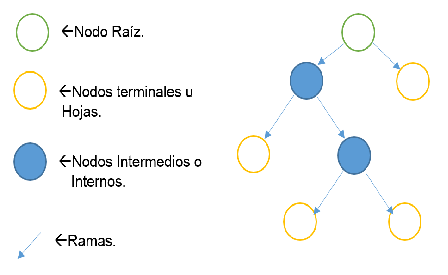
\includegraphics[scale=0.3]{arboles2.png}
\caption{Estructura de un Árbol de Decisión}\label{iamgen:arboldedecisión}
\end{figure} 


\textbf{Nodos Internos}: Se generan cuando los objetos en el pertenecen a dos o más clases.

\textbf{Nodos Hoja}: Se hacen corresponder con una clase concreta.

Ventajas de los árboles de decisión:
\begin{itemize}
\item Aportan una explicación a la clasificación.
\item Son capaces de extraer una estructura que representa, el concepto o patrón de comportamiento que hay asociado a la muestra sobre lo que se ha inducido.

\end{itemize}

Los \textbf{AD} nos ayudan a representar la información de manera jerárquica y de esta manera ver en qué clase se encuentra un atributo de una instancia, de tal manera que va buscando el atributo con mayor ganancia y ese es el que se considera para que entre como rama en un nivel del árbol y va descendiendo hasta que llega a clasificar un atributo correctamente, este tipo de método requiere que se conozca cierta información como la ganancia y entropía de cada subconjunto a evaluar, la  entropía se refiere al número de instancias que clasifican dentro de cada uno de los valores de la clase. La clasificación final de una instancia depende de las condiciones que se van siguiendo desde la raíz del árbol hasta el final, se requiere evaluar un atributo dentro de todos sus posibles valores y el que tenga la mayor ganancia clasifica, existen formas distintas de clasificar los atributos cuando son numéricos se requiere aplicar un criterio de partición para poder evaluar este tipo de atributos, ya que de esto dependerá en parte que se elabore un buen árbol se deben añadir los hijos resultantes de cada partición las particiones al menos deben separar ejemplos en distintos hijos, con lo que la cordialidad de los nodos irá disminuyendo a medida que se desciende en el árbol. Entre más particiones se tenga los árboles que se creen serán más explícitos y probablemente precisos. Para cada nodo que se coloca en el árbol se debió haber evaluado una atributo especifico y este no debe repetirse más adelante, es decir ya no se puede evaluar en niveles de abajo ya que se estaría repitiendo y seria como si se ciclara, cada hoja nos indica en donde se están clasificando esas instancias, las instancias que aún no se sabe dónde clasifican van bajando en los niveles del árbol. 
En weka el algoritmo J4.8. nos permite trabajar con con valores continuos para los atributos, separando los posibles resultados en dos ramas. Los árboles son mas pequeños porque cada hoja no cubre una clase en particular sino una distribución de clases. Particiones realizadas recursivamente, según la estrategia de profundidad-primero (depth-first). Antes de cada partición de datos, el algoritmo considera todas las pruebas posibles que pueden dividir el conjunto de datos y selecciona la prueba que resulta en la mayor ganancia de información o en la mayor proporción de ganancia de información. Cabe resaltar que para cada atributo continuo se realiza una prueba binaria respecto a a los posibles valores que puede tomar el atributo en los datos.
Para realizar este método se comienza por elegir un atributo de prueba, esto se hace mediante la aplicación de la fórmula de entropía, sea una función de ganancia de información, es una propiedad estadística que mide como clasifica un atributo X a los objetos del conjunto de entrenamiento (E).
Entropía es la efectividad de un atributo para subdividir un conjunto de ejemplos en subconjuntos\cite{Datamining}.
\begin{equation}
\left[ E\right] =info(E)=-\sum_{(f=1)}^{(k)}Pj\log_2Pj
\end{equation}
Primero por subconjunto o por nodo y también se debe obtener la entropía general de ese conjunto.
Una vez que se tiene la entropía se calcula la efectividad.
\begin{equation}
SE(X,C,A_i)=-\sum_{(V_ij\epsilon A_i)}\frac{|\left[ A_i(C)=V_ij\right] |}{|X|}I(\left[ A_i(C)=V_ci\right] ,C)
\end{equation}
Después se obtiene la ganancia.
\begin{equation}
G(|X|,C,A_i)=I(X,C)-E(X,C,A_i)
\end{equation}
El criterio de ganancia selecciona el test que maximice esta ganancia de información (información 
mutua entre el test X y la clase)



\section{Método de Redes Neuronales (RD)}
Las \textbf{RN} tratan de emular en un medio sintético (maquina, computadora, algoritmo, regla) la forma en la que un ser humano llega a una conclusión mediante el uso de \textbf{RN}.
Este método sirven como un clasificador de clases por lo tanto cuando se tiene un gran número de datos y variables, una base de datos en la cual se tiene la evolución de esas variables y se tiene un gran poder de cálculo se puede aplicar este método de clasificación.
Una \textbf{RN} tiene la capacidad de aprendizaje esto se realiza mediante el proceso de entrenamiento, este proceso consiste en ir modificando los pesos para cada entrada de las respectivas neuronas en cada iteración hasta encontrar los pesos adecuados, esto hace que se encuentre los pesos para que se cumpla o se verifique el patrón de entrada-salida.
En la arquitectura de una \textbf{RN} se requiere saber el número de neuronas, las entradas que se necesitan, cuántas familias o clases se tiene, y la  función de activación que coloca a esta neurona en un estado activo 1, existen diferentes funciones de activación como: Hardlim, Satlins, sigmoidal, y otras. 
La forma más sencilla o básica de una \textbf{RN} es el perceptron simple, el cual es una configuración de neuronas las cuales están en una sola línea según lo que requiera el problema\cite{Datamining}.
se requiere tener un patrón de entradas y salidas con el cual se va entrenar la \textbf{RN}, por ejemplo puede ser la función de conjunción o disyunción, la función básica para el cálculo de las salidas de una red neuronal es, por ejemplo:
\begin{equation}
S=f(\sum_{(i=1)}^{(n)}e*W+O)
\end{equation}

e= entradas
W= pesos (se inician aleatoriamente).
O=ófsets o vías.
Existe también formas de entrenar una \textbf{RN} y de encontrar los métodos, uno de ellos es Backpropagation o mejor llamada en español la propagación hacia delante consiste en agregar un incremento, calcular el incremento de los nodos, posteriormente calcular el peso final, que no es más que el peso inicial sumado al incremento del peso. 
Estas salidas se introducen en la función de activación y se activa o no se compara el resultado con el patrón deseado.
Existen diversos criterios para realizar la parada de este algoritmo, uno de ellos es el número de iteraciones que se desea y otro es que ya se haya acabado de clasificar todas las instancias. 

\section{Método de K-Vecinos (KV)}
También llamado la regla del vecino más cercano, en un principio este algoritmo se basaba en que un objeto podía pertenecer  a la clase a la que más se pareciera, así que la clase más cercana era la etiqueta de clase que se asignaba al objeto nuevo. 
Una variante de este método es KV (K-Vecinos), en él se asigna la clase mayoritaria entre los k-vecinos más cercanos. Si hay un empate se aplica el criterio donde se asigna al objeto s clasificar la clase que tenga el primer vecino más cercano entre las empatadas.
Este método consiste en medir la distancia entre objetos de acuerdo al valor de los atributos numéricos, la distancia se mide de acuerdo a la fórmula que se desee, existen diferentes tipos de distancia, en este algoritmo se mide la distancia de un objeto al resto de los objetos del conjunto de entrenamiento, luego se toman los resultados de los \textbf{KN} más cercanos, es decir aquellos cuya distancia a dicho objeto de entrenamiento sea menor, y  de acuerdo a la etiqueta de clase que tengan la mayoría de los \textbf{KN} más cercanos esa será la clase asignada al nuevo objeto a clasificar\cite{Datamining}.


En este método existen diferentes tipos de distancias que se pueden aplicar, como lo son:

La formula para la distancia euclidiana es la siguiente:
\begin{equation}
d(x,y)=\sqrt{\sum_{i=1}^{n}(X_i-Y_i)^2}
\end{equation}

Esta distancia fue la una de las que se utilizaron en el curso y la cual se utilizó para aplicar el método de K-Vecinos sobre los conjuntos de entrenamiento.



\section{Método de Máquinas de Vectores de Soporte (MVS)}

La \textbf{MKV} fue diseñada para la clasificación binaria, éste es un modelo predictivo de aprendizaje supervisado, utiliza planos de decisión, es decir define una frontera de decisión para clasificar a los objetos de entrenamiento, para conjuntos linealmente separables. Para esto se calculan los hiperplanos que son las fronteras de decisión entre cada clase, que son positiva o negativa, éste es un método de aprendizaje supervisado. 
Para clasificar un nuevo objeto de entrenamiento se calcula el tamaño del vector dependiendo de los atributos que se tengan y multiplica el alfa por los respectivos vectores de los objetos de entrenamiento que se toman como vectores de soporte, luego el valor obtenido de la sumatoria de estos vectores se multiplica por el vector de dicho objeto de entrenamiento de los atributos  y  por su respectiva clase que es positiva o negativa, enseguida se despeja a b para cada vector, luego se obtiene el promedio de las b despejadas y el resultado de esa b se multiplica por el vector de atributos del objeto de entrenamiento tomado como vector de soporte y por la clase. Esto se realiza para la clasificación de un nuevo objeto y si el resultado es negativo el nuevo objeto a clasificar clasifica en la clase de los negativos y si es positivo en los positivos.
%%%%%%%%%%%%%%
% Capítulo 2 %
%%%%%%%%%%%%%%
\chapter{Weka}
%%%%%%%%%%%%%%%%%%%%%%%%%%
%Sección del capítulo 2%
%%%%%%%%%%%%%%%%%%%%%%%%%%

Es un software que funciona como una  máquina de aprendizaje automático,  oficialmente es un  Entorno para Análisis del Conocimiento creado originalmente en 1993 como un proyecto en la Universidad de Waikato, Nueva Zelanda.

Weka tiene grandes ventajas ya que es un software de código abierto y  está programado en java que es un lenguaje multiplataforma (entre sus múltiples ventajas), y aunque no hay una documentación muy amplia del software resulta bastante intuitivo para el usuario. 

Weka posee una extensa  colección de algoritmos de Máquinas de conocimiento desarrollados para entre otras aplicaciones para la minería de datos. Además Weka contiene las herramientas necesarias para realizar transformaciones sobre los datos, tareas de clasificación, regresión, clustering, asociación y visualización. Weka está diseñado como una herramienta orientada a la extensibilidad esto en parte se debe al hecho está programada en java lo que facilita esta característica en el software\cite{Documentación de Weka}.

Para su funcionamiento Weka recibe un archivo que contiene la base de datos que será utilizada como el conjunto de entrenamiento para la máquina de aprendizaje, el formato que deben tener todos los archivos que son introducidos en Weka es  .arff, la estructura de este formato está compuesta por tres partes: 



%%%%

\textbf{La declaración \textit{@relation}}


El nombre de la relación se define como la primera línea en el archivo ARFF . El formato es:

    \textit{@relation} <nombre-relación>
   
donde <nombre-relacion> es una cadena de textos. La cadena no debe contener espacios.


\textbf{La declaración\textit{@attribute}}


Cada atributo en el conjunto de datos tiene su propia declaración de \textit{@attribute} que define de forma exclusiva el nombre de ese atributo y su tipo de datos. 
El orden de los atributos se declaran indicando la posición de la columna en la sección de datos del archivo. 
El formato para la declaración del \textit{@attribute} es:

    @attribute <tipoDeDatos> <nombre-atributo>
   
donde el <nombre-atributo> debe comenzar con un carácter alfabético. Si los espacios se van a incluir en el nombre y luego el nombre completo debe ser citado.

Con <tipoDeDatos> indicaremos el tipo de dato para este atributo (o columna) que puede ser:
\begin{itemize}
\item string (texto).
\item date [<date-format>] (fecha). En <date-format> indicaremos el formato de la fecha, que será del tipo "yyyy-MM-dd'T'HH:mm:ss".
\item numeric (numérico)
\item <nominal-specification>. Estos son tipos de datos definidos por nosotros mismos.
\end{itemize}

\textbf{La declaración\textit{@data}}


En esta sección incluiremos los datos propiamente dichos. Separaremos cada columna por comas y todas filas deberán tener el mismo número de columnas, número que coincide con el de declaraciónes @attribute que añadimos en la sección anterior.
Si no disponemos de algún dato, colocaremos un signo de interrogación (?) en su lugar. El separador de decimales tiene que ser obligatoriamente el punto y las cadenas de tipo string tienen que estar entre comillas simples\cite{Waikaton}.


\textbf{Explorer}

Interfaz básico para usar el conjunto de algoritmos que ofrece WEKA (clasificación, clustering, reglas de asociación, selección de atributos y visualización).

\textbf{Experimenter}

Interfaz gráfico para automatizar baterías de experimentos.

\textbf{Knowledge Flow}

Interfaz gráfico para diseñar flujos y procesos donde se combinen varios componentes para conformar aplicaciones complejas.

\textbf{Simple CLI}

Acceso los algoritmos de WEKA desde un interfaz de línea de comandos.
Para realizar esta práctica se empleará el interfaz Explorer (ver presentación PPT), si se hacen las pruebas ''manuales'', o el interfaz Experimenter, si se desean automatizar las pruebas.

Las funcionalidades del interfaz Explorer se organizan en 6 pestañas:

\textbf{Preprocess}

Carga de los datasets a emplear y procesamiento previo a la aplicación de los algoritmos de aprendizaje
Permite cargar datos desde ficheros ARFF, ficheros CSV y bases de datos (mediante JDBC).


\textbf{Classify}

Interfaz de experimentación con algoritmos de clasificación
Permite seleccionar un clasificador (botón [Choose]) y configurar sus parámetros (pulsando sobre el nombre del algoritmo)

Permite especificar el método de evaluación (Test options)

El resultado de aplicar el clasificador elegido será puesto a prueba de acuerdo con las opciones 
que se establecen haciendo clic en el cuadro de Test options. 

Hay cuatro modos de prueba:
 
\begin{itemize}
\item \textit{training set}: esta opción evalúa el clasificador sobre el mismo conjunto 
sobre el que se construye el modelo predictivo para determinar el error, que 
en este caso se denomina "error de resustitución". Por tanto, esta opción 
puede proporcionar una estimación demasiado optimista del 
comportamiento del clasificador, al evaluarlo sobre el mismo conjunto sobre 
el que se hizo el modelo. 
\item \textit{Supplied test set}: evaluación sobre conjunto independiente. Esta opción 
permite cargar un conjunto nuevo de datos. Sobre cada dato se realizará 
una predicción de clase para contar los errores. 
\item \textit{Cross-validation}: evaluación con validación cruzada. Esta opción es la 
más elaborada y costosa. Se realizan tantas evaluaciones como se indica 
en el parámetro Folds. Se dividen las instancias en tantas carpetas como 
indica este parámetro y en cada evaluación se toman las instancias de cada 
carpeta como datos de test, y el resto como datos de entrenamiento para 
construir el modelo. Los errores calculados son el promedio de todas las 
ejecuciones. 
\item \textit{Percentage split}: esta opción divide los datos en dos grupos, de acuerdo 
con el porcentaje indicado (\%). El valor indicado es el porcentaje de 
instancias para construir el modelo, que a continuación es evaluado sobre 
las que se han dejado aparte. Cuando el Instancias es 
suficientemente elevado, esta opción es suficiente para estimar con 
precisión las prestaciones del clasificador en el dominio\cite{Tutorial de Weka}. 
\end{itemize}


Permite establecer el atributo clase sobre el que realizar el aprendizaje
Muestra los resultados del proceso entrenamiento-evaluación

\textbf{Cluster}

Interfaz de experimentación con algoritmos de clustering

\textbf{Associate}

Interfaz de experimentación con algoritmos para aprendizaje de reglas de asociación

\textbf{Select attributes}

Interfaz de experimentación con algoritmos de selección de atributos

\textbf{Visualize}

Interfaz para la visualización de datasets, relaciones entre atributos, etc \cite{Uvigo}.
%%%%%%%%%%%%%%
% Capítulo 3 %
%%%%%%%%%%%%%%
\chapter{Resultados Experimentales}
%%%%%%%%%%%%%%%%%%%%%%%%%%
%Sección del capítulo    %
%%%%%%%%%%%%%%%%%%%%%%%%%%

%%%%%%%%%%%%%%%%%%%
%    1. Abalone   %
%%%%%%%%%%%%%%%%%%%
\section{Abalone}
%%%%%%%%%%%%%%%%%%%%%%%%%%
%Sección de  Abalone     %
%%%%%%%%%%%%%%%%%%%%%%%%%%
La base de datos Abalone es originaria de un estudio titulado "La población biológica de Abalone (especie Haliotis) en Tasmania.", de la división de recursos de la marina y el laboratorio de investigación marina.
La base de datos contiene información que predice la edad de Abalone, dadas sus medidas físicas. 
La edad de Abalone es determinada al cortar la coraza por el cono, creando una mancha y contando el número de anillos utilizando un microscopio para ello; es una actividad aburrida y que consume mucho tiempo \cite{Datasets}.
%%%%%%%%%%%%%%%%%%%%%%%%%%%%%%%%%%%%%%%%%%%%
% Tabla de Instancias y número de atributos%
%%%%%%%%%%%%%%%%%%%%%%%%%%%%%%%%%%%%%%%%%%%%
\begin{table}[H]
\centering % es usado para centrar la tabla
\begin{tabular}{c c}
% columnas centradas (2 columnas)
\hline\hline %inserts double horizontal lines
Instancias & Atributos \\ [0.5ex]
% inserta tablas
%heading
\hline % Inserta una linea horizontal
4177 & 9 \\ [1ex] % [1ex] Agrega un espacio vertical
\hline %Inserta una linea
\end{tabular}
\label{center:Abaloneia} % Es usado para referise a esta tabla en el texto
\caption{Número de Instancias y Atributos del conjunto de datos de Abalone} % titulo de la tabla
\end{table}
%%%%%%%%%%%%%%%%%%%%
% Finaliza la tabla%
%%%%%%%%%%%%%%%%%%%%
%%%%%%%%%%%%%%%%%%%%%%%
% Atributos de Abalone%
%%%%%%%%%%%%%%%%%%%%%%%
\begin{table}[H]

\centering % es usado para centrar la tabla
\begin{tabular}{c c c}
% columnas centradas (2 columnas)
\hline\hline %inserts double horizontal lines
Atributo & Tipo & Dominio \\ [0.5ex]
% inserta tablas
%heading
\hline % Inserta una linea horizontal
sexo & Categórico & M, F, I\\ [1ex] % [1ex] Agrega un espacio vertical
longitud & Real & 0.45, 0.33, 0.256, …\\ [1ex] % [1ex] Agrega un espacio vertical
Diámetro & Real & 0.365, 0.600, 0.666, etc.\\ [1ex] % [1ex] Agrega un espacio vertical
Altura & Real & 0.4755, 0.420, 0.1366…\\ [1ex] % [1ex] Agrega un espacio vertical
Peso completo & Real. & 1.2, 0.4678, …\\ [1ex] % [1ex] Agrega un espacio vertical
Peso sin concha & Real. & 0.365, 0.444, 0.3200, …\\ [1ex] % [1ex] Agrega un espacio vertical
Peso visceras & Real. & 0.4755, 0.45, 0.33, …\\ [1ex] % [1ex] Agrega un espacio vertical
Peso coraza & Real. & 0.4755, 0.4005, 0.3233, …\\ [1ex] % [1ex] Agrega un espacio vertical
clase & Numérico. & 4,5,10, 19,… etc.\\ [1ex] % [1ex] Agrega un espacio vertical
\hline %Inserta una linea
\end{tabular}
\label{table:Abalonea} % Es usado para referise a esta tabla en el texto
\caption{Atributos del conjunto de datos de Abalone} % titulo de la tabla
\end{table}
%%%%%%%%%%%%%%%%%%%%
% Finaliza la tabla%
%%%%%%%%%%%%%%%%%%%%

\begin{figure}[H]
    \centering
    \begin{tikzpicture}
   
    \begin{axis}[
        nodes near coords,
     ylabel=Instancias clasificadas correctamente (\%), 
    xlabel=Métodos de clasificación,     
            symbolic x coords={NB,AD,RN,MVS,KV1,KV3,KV5},
            xtick=data
          ]
    \addplot[ybar,fill=blue] coordinates {
                (NB, 23.8449)
                (AD, 21.1635)
                (RN, 26.5520)                
                (MVS,25.2574)
                (KV1,20.5411)
                (KV3,21.8578)
                (KV5,23.3661)
            };         
    \end{axis}
    \end{tikzpicture}  
    \caption{Porcentajes de clasificación correcta del conjunto de datos de Abalone}
    \label{graph:graficocdAbalone} % Es usado para referise a un gráfico
\end{figure}
\begin{figure}[H]
 	\centering
    \begin{tikzpicture}
   
    \begin{axis}[
                nodes near coords,
     ylabel= Tiempo de ejecución (Segundos), 
    xlabel=Métodos de clasificación, 
            symbolic x coords={NB,AD,RN,MVS,KV1,KV3,KV5},
            xtick=data
          ]
    \addplot[ybar,fill=blue] coordinates {
                (NB, .5)
                (AD, 3)
                (RN, 334)                
                (MVS, 17)
                (KV1,2)
                (KV3,1)
                (KV5,1)
            };
    \end{axis}
    \end{tikzpicture}
    \caption{Tiempos del procesamiento del conjunto de datos de Abalone}    
    \label{graph:graficotAbalone} % Es usado para referise a un gráfico
\end{figure}


%%%%%%%%%%%%%%%%%%%%%%%%
% 5. Conclusiones %
%%%%%%%%%%%%%%%%%%%%%%%%

%%%%%%%%%%%%%%%
%Conclusiones %
%%%%%%%%%%%%%%%
Los resultados generales de la clasificación se muestran en la Figura \ref{graph:graficocdAbalone}  donde se puede ver el porcentaje de clasificación correcta
que obtiene cada método de clasificación utilizada. la 	Figura \ref{graph:graficotAbalone} muestra por su parte los resultados del tiempo de procesamiento empleado por cada algoritmo mostrado en segundos. Estos resultados son un porcentaje de la clasificación del conjunto de datos Abalone aplicado a 5 métodos de clasificación. 
De acuerdo a los métodos que tuvieron un mayor porcentaje de clasificación de instancias, se puede apreciar que para este caso existen dos métodos con un indice alto de clasificación fueron Redes Neuronales y Máquinas de Soporte de Vectores. Por otro lado, es importante considerar el tiempo que tardaron en clasificar estos métodos, como se puede apreciar en la Figura \ref{graph:graficotAbalone}, el método de Máquinas de Soporte de Vectores se tardó menos tiempo que el método de Redes Neuronales.
En los demás métodos de clasificación empleados, se observo que su precisión fue similar, sin embargo su porcentaje de error de clasificación fue mayor a los 2 métodos con mayor porcentaje de clasificación correcta, debido a que tenían errores al momento de clasificar, ésto se observa en las matrices de que se obtuvieron en la aplicación de los métodos.
Por lo tanto, para clasificar este conjunto de datos siempre será mejor utilizar el método de Maquinas de Vectores de Soporte debido a que tuvo un porcentaje considerable de clasificación y el tiempo que demoro en clasificar es mínimo en comparación al del otro método. 

$  $
%%%%%%%%%%%%%%%%%%%%
%    2. Rookpawn   %
%%%%%%%%%%%%%%%%%%%%
\section{Rookpawn}
%%%%%%%%%%%%%%%%%%%%%%%%%%
%Sección de  Rookpawn    %
%%%%%%%%%%%%%%%%%%%%%%%%%%
\begin{quotation}
La base de datos de Rey Rook y Rey Pawn (ajedrez) fue donada por Rob Holte y generada y descrita por Alen Shapiro. La base de datos fue suministrada a Holte por Peter Clark del Instituto Turing en Glasgow\cite{Datasets}.
%%%%%%%%%%%%%%%%%%%%%%%%%%%%%%%%%%%%%%%%%%%%%%%%%%%%%%%
% Atributos de Abalone					        	  %
%%%%%%%%%%%%%%%%%%%%%%%%%%%%%%%%%%%%%%%%%%%%%%%%%%%%%%%
\end{quotation}
%%%%%%%%%%%%%%%%%%%%%%%%%%%%%%%%%%%%%%%%%%%%%%%%%%%%%%%
% Tabla de Instancias y número de atributos %
%%%%%%%%%%%%%%%%%%%%%%%%%%%%%%%%%%%%%%%%%%%%%%%%%%%%%%%
\begin{table}[H]
\caption{Número de Instancias y Atributos Rookpawn} % titulo de la tabla
\centering % es usado para centrar la tabla
\begin{tabular}{c c}
% columnas centradas (2 columnas)
\hline\hline %inserts double horizontal lines
Instancias & Atributos \\ [0.5ex]
% inserta tablas
%heading
\hline % Inserta una linea horizontal
3196 & 37 \\ [1ex] % [1ex] Agrega un espacio vertical
\hline %Inserta una linea
\end{tabular}
\label{table:rookpawnia} % Es usado para referise a esta tabla en el texto
\end{table}
%%%%%%%%%%%%%%%%%%%%
% Finaliza la tabla%
%%%%%%%%%%%%%%%%%%%%
\newpage 

\begin{table}[H]
\caption{Atributos de Rookpawn} % titulo de la tabla
\centering % es usado para centrar la tabla
\begin{tabular}{c c c}
% columnas centradas (3 columnas)
\hline\hline %inserts double horizontal lines
Atributo & Tipo & Dominio \\ [0.5ex]
% inserta tablas
%heading
\hline % Inserta una linea horizontal
 bkblk & Categórico & {f,t}\\ [1ex] % [1ex] Agrega un espacio vertical
 bknwy & Categórico & {f,t}\\ [1ex] % [1ex] Agrega un espacio vertical
 bkon8 & Categórico & {f,t}\\ [1ex] % [1ex] Agrega un espacio vertical
 bkona & Categórico & {f,t}\\ [1ex] % [1ex] Agrega un espacio vertical
 bkspr & Categórico & {f,t}\\ [1ex] % [1ex] Agrega un espacio vertical
 bkxbq & Categórico & {f,t}\\ [1ex] % [1ex] Agrega un espacio vertical
 bkxcr & Categórico & {f,t}\\ [1ex] % [1ex] Agrega un espacio vertical
 bkxwp & Categórico & {f,t}\\ [1ex] % [1ex] Agrega un espacio vertical
 blxwp & Categórico & {f,t}\\ [1ex] % [1ex] Agrega un espacio vertical
 bxqsq & Categórico & {f,t}\\ [1ex] % [1ex] Agrega un espacio vertical
 cntxt & Categórico & {f,t}\\ [1ex] % [1ex] Agrega un espacio vertical
 dsopp & Categórico & {f,t}\\ [1ex] % [1ex] Agrega un espacio vertical
 dwipd & Categórico & {l,g}\\ [1ex] % [1ex] Agrega un espacio vertical
 hdchk & Categórico & {f,t}\\ [1ex] % [1ex] Agrega un espacio vertical
 katri & Categórico & {n,w,b}\\ [1ex] % [1ex] Agrega un espacio vertical
 mulch & Categórico & {f,t}\\ [1ex] % [1ex] Agrega un espacio vertical
 qxmsq & Categórico & {f,t}\\ [1ex] % [1ex] Agrega un espacio vertical
 r2ar8 & Categórico & {t,f}\\ [1ex] % [1ex] Agrega un espacio vertical
 reskd & Categórico & {f,t}\\ [1ex] % [1ex] Agrega un espacio vertical
 reskr & Categórico & {f,t}\\ [1ex] % [1ex] Agrega un espacio vertical
 rimmx & Categórico & {f,t}\\ [1ex] % [1ex] Agrega un espacio vertical
 rkxwp & Categórico & {f,t}\\ [1ex] % [1ex] Agrega un espacio vertical
 rxmsq & Categórico & {f,t}\\ [1ex] % [1ex] Agrega un espacio vertical
 simpl & Categórico & {f,t}\\ [1ex] % [1ex] Agrega un espacio vertical
 skach & Categórico & {f,t}\\ [1ex] % [1ex] Agrega un espacio vertical
 skewr & Categórico & {t,f}\\ [1ex] % [1ex] Agrega un espacio vertical
 skrxp & Categórico & {f,t}\\ [1ex] % [1ex] Agrega un espacio vertical
 spcop & Categórico & {f,t}\\ [1ex] % [1ex] Agrega un espacio vertical
 stlmt & Categórico & {f,t}\\ [1ex] % [1ex] Agrega un espacio vertical
 thrsk & Categórico & {f,t}\\ [1ex] % [1ex] Agrega un espacio vertical
 wkcti & Categórico & {f,t}\\ [1ex] % [1ex] Agrega un espacio vertical
 wkna8 & Categórico & {f,t}\\ [1ex] % [1ex] Agrega un espacio vertical
 wknck & Categórico & {f,t}\\ [1ex] % [1ex] Agrega un espacio vertical
 wkovl & Categórico & {t,f}\\ [1ex] % [1ex] Agrega un espacio vertical
 wkpos & Categórico & {t,f}\\ [1ex] % [1ex] Agrega un espacio vertical
 wtoeg & Categórico & {n,t}\\ [1ex] % [1ex] Agrega un espacio vertical
 clase & Categórico & {won,nowin}\\ [1ex] % [1ex] Agrega un espacio vertical
\hline %Inserta una linea
\end{tabular}
\label{table:rookpawn} % Es usado para referise a esta tabla en el texto
\end{table}
%%%%%%%%%%%%%%%%%%%%
% Finaliza la tabla%
%%%%%%%%%%%%%%%%%%%%




\begin{figure}[H]
 \centering
    \begin{tikzpicture}
   
        \begin{axis}[
                nodes near coords,
     ylabel=Instancias clasificadas correctamente (\%), 
    xlabel=Métodos de clasificación,    
            symbolic x coords={NB,AD,RN,MVS,KV1,KV3,KV5},
            xtick=data
          ]
          \addplot[ybar,fill=blue] coordinates {
                (NB, 88.3292)
                (AD, 99.4368)
                (RN, 99.3116)                
                (MVS,95.6195)
                (KV1,96.2766)
                (KV3,96.4956)
                (KV5,96.0263)
            };
            


        \end{axis}
    \end{tikzpicture}
     \caption{Porcentajes de clasificación correcta del conjunto de datos de Rookpawn}
     \label{graph:graficocrookpawn}
\end{figure}

\begin{figure}[H]
 \centering
    \begin{tikzpicture}
   
        \begin{axis}[
                nodes near coords,
     ylabel=Tiempo de ejecución (Segundos), 
    xlabel=Métodos de clasificación,    
            symbolic x coords={NB,AD,RN,MVS,KV1,KV3,KV5},
            xtick=data
          ]
          \addplot[ybar,fill=blue] coordinates {
                (NB, 0.1)
                (AD, 0.8)
                (RN, 235)                
                (MVS, 7)
                (KV1,40)
                (KV3,45)
                (KV5,46)
            };
            


        \end{axis}
    \end{tikzpicture}
     \caption{Tiempos del procesamiento del conjunto de datos de Rookpawn}
     \label{graph:graficotrookpawn}
\end{figure}





%%%%%%%%%%%%%%%%%%%%%%%%
% 5. Conclusiones %
%%%%%%%%%%%%%%%%%%%%%%%%

Los resultados generales de la clasificación se muestran en la Figura  \ref{graph:graficocrookpawn}  donde se puede ver el porcentaje de clasificación correcta
que obtiene cada método de clasificación utilizada. la 	Figura \ref{graph:graficotrookpawn} muestra por su parte los resultados del tiempo de procesamiento empleado por cada algoritmo mostrado en segundos. Estos resultados son un porcentaje de la clasificación del conjunto de datos Rookpawn aplicado a 5 métodos de clasificación. 
De acuerdo a los métodos que tuvieron un mayor porcentaje de clasificación de instancias, se puede apreciar que para este caso existen dos métodos con un indice alto de clasificación fueron Árboles de Decisión y Redes Neuronales. Por otro lado, es importante considerar el tiempo que tardaron en clasificar estos métodos, como se puede apreciar en la Figura \ref{graph:graficotrookpawn}, el método de Árboles de Decisión se tardó menos tiempo que el método de Redes Neuronales. En los demás métodos de clasificación empleados, se observo que su precisión fue similar, sin embargo su porcentaje de error de clasificación fue mayor a los 2 métodos con mayor porcentaje de clasificación correcta, debido a que tenían errores al momento de clasificar, ésto se observa en las matrices de que se obtuvieron en la aplicación de los métodos.
Por lo tanto, para clasificar este conjunto de datos siempre será mejor utilizar el método de Árboles de Decisión debido a que tuvo un porcentaje considerable de clasificación y el tiempo que demoro en clasificar es mínimo en comparación al del otro método. 

\newpage
%%%%%%%%%%%%%%%%%%%%%%%%%%%%%
%    3. Segmentación de Piel   %
%%%%%%%%%%%%%%%%%%%%%%%%%%%%%
\section{Segmentación de Piel}
%%%%%%%%%%%%%%%%%%%%%%%%%%%%%%%%%%%%%%
%Sección de  Segmentación de Piel    %
%%%%%%%%%%%%%%%%%%%%%%%%%%%%%%%%%%%%%%
El conjunto de datos de la piel es recogida por muestreo aleatorio B, G, R valores de imágenes de caras de diferentes grupos de edad (jóvenes, de mediana y edad), grupos de raza (blanco, negro y asiático), y géneros obtenidos de la base de datos y base de datos FERET PAL. Tamaño de la muestra total de aprendizaje es de 245,057; de los cuales 50,859 son las muestras de piel y 194,198 no son muestras de piel\cite{Datasets}.
%%%%%%%%%%%%%%%%%%%%%%%%%%%%%%%%%%%%%%%%%%%%%%%%%%%%%%%
% Tabla de Instancias y número de atributos %
%%%%%%%%%%%%%%%%%%%%%%%%%%%%%%%%%%%%%%%%%%%%%%%%%%%%%%%
\begin{table}[H]
\caption{Número de Instancias y Atributos Segmentación de Piel} % titulo de la tabla
\centering % es usado para centrar la tabla
\begin{tabular}{c c}
% columnas centradas (2 columnas)
\hline\hline %inserts double horizontal lines
Instancias & Atributos \\ [0.5ex]
% inserta tablas
%heading
\hline % Inserta una linea horizontal
245057 & 4 \\ [1ex] % [1ex] Agrega un espacio vertical
\hline %Inserta una linea
\end{tabular}
\label{table:segmentacionpielia} % Es usado para referise a esta tabla en el texto
\end{table}
%%%%%%%%%%%%%%%%%%%%
% Finaliza la tabla%
%%%%%%%%%%%%%%%%%%%%
%%%%%%%%%%%%%%%%%%%%%%%%%%%%%%%%%%%%%%%%%%%%%%%%%%%%%%%
% Atributos de segmentacion piel       	              %
%%%%%%%%%%%%%%%%%%%%%%%%%%%%%%%%%%%%%%%%%%%%%%%%%%%%%%%
\begin{table}[H]
\caption{Atributos de Segmentación de Piel} % titulo de la tabla
\centering % es usado para centrar la tabla
\begin{tabular}{c c c}
% columnas centradas (3 columnas)
\hline\hline %inserts double horizontal lines
Atributo & Tipo & Dominio \\ [0.5ex]
% inserta tablas
%heading
\hline % Inserta una linea horizontal
R & Entero & 0,..255\\ [1ex] % [1ex] Agrega un espacio vertical
G & Entero & 0,..255\\ [1ex] % [1ex] Agrega un espacio vertical
B & Entero & 0,..255\\ [1ex] % [1ex] Agrega un espacio vertical
Clase & Categórico & {1,2}\\ [1ex] % [1ex] Agrega un espacio vertical
\hline %Inserta una linea
\end{tabular}
\label{table:segmentacionpiela} % Es usado para referise a esta tabla en el texto
\end{table}
%%%%%%%%%%%%%%%%%%%%
% Finaliza la tabla%
%%%%%%%%%%%%%%%%%%%%



\begin{figure}[H]
 \centering
    \begin{tikzpicture}
   
        \begin{axis}[
                nodes near coords,
     ylabel=Instancias clasificadas correctamente (\%), 
    xlabel=Métodos de clasificación,    
            symbolic x coords={NB,AD,RN,MVS,KV1,KV3,KV5},
            xtick=data
          ]
          \addplot[ybar,fill=blue] coordinates {
                (NB, 92.3936)
                (AD, 99.931)
                (RN, 99.4552)                
                (MVS,92.9021)
                (KV1,99.9588)
                (KV3,99.9555)
                (KV5,99.9506)
            };
            


        \end{axis}
    \end{tikzpicture}
     \caption{Porcentajes de clasificación correcta del conjunto de datos de Segmentación de Piel}
      \label{graph:graficocsegmentacion}
\end{figure}

\begin{figure}[H]
 \centering
    \begin{tikzpicture}
   
        \begin{axis}[
                nodes near coords,
     ylabel=Tiempo de ejecución (Segundos), 
    xlabel=Métodos de clasificación,    
            symbolic x coords={NB,AD,RN,MVS,KV1,KV3,KV5},
            xtick=data
          ]
          \addplot[ybar,fill=blue] coordinates {
                (NB, 0.21)
                (AD, 0.48)
                (RN, 766)                
                (MVS, 4191)
                (KV1,5657 )
                (KV3,6298)
                (KV5,5304)
            };
            


        \end{axis}
    \end{tikzpicture}
     \caption{Tiempos del procesamiento del conjunto de datos de Segmentación de Piel}
     \label{graph:graficotsegmentacion}
\end{figure}




%%%%%%%%%%%%%%%%%%%%%%%%
% 5. Conclusiones %
%%%%%%%%%%%%%%%%%%%%%%%%
Los resultados generales de la clasificación se muestran en la Figura \ref{graph:graficocsegmentacion} donde se puede ver el porcentaje de clasificación correcta que obtiene cada método de clasificación utilizada. la 	Figura \ref{graph:graficotsegmentacion} muestra por su parte los resultados del tiempo de procesamiento empleado por cada algoritmo mostrado en segundos. Estos resultados son un porcentaje de la clasificación del conjunto de datos de Segmentación de Piel aplicado a 5 métodos de clasificación. 
De acuerdo a los métodos que tuvieron un mayor porcentaje de clasificación de instancias, se puede apreciar que para este caso existen dos métodos con un indice alto de clasificación fueron Árboles de Decisión y  K-Vecinos. Por otro lado, es importante considerar el tiempo que tardaron en clasificar estos métodos, como se puede apreciar en la Figura \ref{graph:graficotsegmentacion}, el método de Árboles de Decisión se tardó menos tiempo que el método de  K-Vecinos. En los demás métodos de clasificación empleados, se observo que su precisión fue similar, sin embargo su porcentaje de error de clasificación fue mayor a los 2 métodos con mayor porcentaje de clasificación correcta, debido a que tenían errores al momento de clasificar, ésto se observa en las matrices de que se obtuvieron en la aplicación de los métodos.
Por lo tanto, para clasificar este conjunto de datos siempre será mejor utilizar el método de Árboles de Decisión debido a que obtuvo un porcentaje considerable de clasificación y el tiempo que demoro en clasificar es mínimo en comparación al del otro método. 

\newpage
%%%%%%%%%%%%%%%%%%%%%%%%%%%%%
%    4. Pokerhand   %
%%%%%%%%%%%%%%%%%%%%%%%%%%%%%
\section{Pokerhand}
%%%%%%%%%%%%%%%%%%%%%%%%%%%%%%%%%%%%%%
%Sección de Pokerhand    %
%%%%%%%%%%%%%%%%%%%%%%%%%%%%%%%%%%%%%%
Cada registro es un ejemplo de una mano con cinco cartas procedentes de una baraja de 52. Cada carta se describe el uso de dos atributos (traje y de la fila), para un total de 10 atributos de predicción. Hay un atributo de clase que describe el "Poker Hand". El orden de las cartas es importante, por lo que hay 480 posibles manos Royal Flush\cite{Datasets}.
%%%%%%%%%%%%%%%%%%%%%%%%%%%%%%%%%%%%%%%%%%%%%%%%%%%%%%%
% Tabla de Instancias y número de atributos %
%%%%%%%%%%%%%%%%%%%%%%%%%%%%%%%%%%%%%%%%%%%%%%%%%%%%%%%
\begin{table}[H]
\caption{Número de Instancias y Atributos Pokerhand} % titulo de la tabla
\centering % es usado para centrar la tabla
\begin{tabular}{c c}
% columnas centradas (2 columnas)
\hline\hline %inserts double horizontal lines
Instancias & Atributos \\ [0.5ex]
% inserta tablas
%heading
\hline % Inserta una linea horizontal
184743 & 11 \\ [1ex] % [1ex] Agrega un espacio vertical
\hline %Inserta una linea
\end{tabular}
\label{table:pokerhandia} % Es usado para referise a esta tabla en el texto
\end{table}
%%%%%%%%%%%%%%%%%%%%
% Finaliza la tabla%
%%%%%%%%%%%%%%%%%%%%
%%%%%%%%%%%%%%%%%%%%%%%%%%%%%%%%%%%%%%%%%%%%%%%%%%%%%%%
% Atributos de pokerhand            	              %
%%%%%%%%%%%%%%%%%%%%%%%%%%%%%%%%%%%%%%%%%%%%%%%%%%%%%%%
\begin{table}[H]
\caption{Atributos de Pokerhand} % titulo de la tabla
\centering % es usado para centrar la tabla
\begin{tabular}{c c c}
% columnas centradas (3 columnas)
\hline\hline %inserts double horizontal lines
Atributo & Tipo & Dominio \\ [0.5ex]
% inserta tablas
%heading
\hline % Inserta una linea horizontal
juegocarta1 & real &  1,..4\\ [1ex] % [1ex] Agrega un espacio vertical
posicioncarta1 & real & 1,..13\\ [1ex] % [1ex] Agrega un espacio vertical
juegocarta2 & real & 1,..4\\ [1ex] % [1ex] Agrega un espacio vertical
posicioncarta2 & real & 1,..13\\ [1ex] % [1ex] Agrega un espacio vertical
juegocarta3 & real & 1,..4\\ [1ex] % [1ex] Agrega un espacio vertical
posicioncarta3 & real & 1,..13\\ [1ex] % [1ex] Agrega un espacio vertical
juegocarta4 & real & 1,..4\\ [1ex] % [1ex] Agrega un espacio vertical
posicioncarta4 & real & 1,..13\\ [1ex] % [1ex] Agrega un espacio vertical
juegocarta5 & real& 1,..4\\ [1ex] % [1ex] Agrega un espacio vertical
posicioncarta5 & real & 1,..13\\ [1ex] % [1ex] Agrega un espacio vertical
clase & Categórico & 0,..9\\ [1ex] % [1ex] Agrega un espacio vertical
\hline %Inserta una linea
\end{tabular}
\label{table:pokerhanda} % Es usado para referise a esta tabla en el texto
\end{table}
%%%%%%%%%%%%%%%%%%%%
% Finaliza la tabla%
%%%%%%%%%%%%%%%%%%%%



\begin{figure}[H]
 \centering
    \begin{tikzpicture}
   
        \begin{axis}[
                nodes near coords,
     ylabel=Instancias clasificadas correctamente (\%), 
    xlabel=Métodos de clasificación,    
            symbolic x coords={NB,AD,RN,MVS,KV1,KV3,KV5},
            xtick=data
          ]
          \addplot[ybar,fill=blue] coordinates {
                (NB, 50.1226)
                (AD, 65.104)
                (RN, 53.4478)                
                (MVS, 50.1226)
                (KV1, 48.0668)
                (KV3, 51.117)
                (KV5, 52.3257)
            };
            


        \end{axis}
    \end{tikzpicture}
     \caption{Porcentajes de clasificación correcta del conjunto de datos de Pokerhand}
     \label{graph:graficocpokerhand}
\end{figure}

\begin{figure}[H]
 \centering
    \begin{tikzpicture}
   
        \begin{axis}[
                nodes near coords,
     ylabel=Tiempo de ejecución (Segundos), 
    xlabel=Métodos de clasificación,    
            symbolic x coords={NB,AD,RN,MVS,KV1,KV3,KV5},
            xtick=data
          ]
          \addplot[ybar,fill=blue] coordinates {
                (NB, 39)
                (AD, 1800)
                (RN, 5750)                
                (MVS, 22531)
                (KV1,1000)
                (KV3,900)
                (KV5,900)
            };
            


        \end{axis}
    \end{tikzpicture}
     \caption{Tiempos del procesamiento del conjunto de datos de Pokerhand}
       \label{graph:graficotpokerhand}
\end{figure}




%%%%%%%%%%%%%%%%%%%%%%%%
% 5. Conclusiones %
%%%%%%%%%%%%%%%%%%%%%%%%

Los resultados generales de la clasificación se muestran en la Figura  \ref{graph:graficocpokerhand} donde se puede ver el porcentaje de clasificación correcta que obtiene cada método de clasificación utilizada. la 	Figura \ref{graph:graficotpokerhand} muestra por su parte los resultados del tiempo de procesamiento empleado por cada algoritmo mostrado en segundos. Estos resultados son un porcentaje de la clasificación del conjunto de datos Pokerhand aplicado a 5 métodos de clasificación. De acuerdo a los métodos que tuvieron un mayor porcentaje de clasificación de instancias, se puede apreciar que para este caso existen dos métodos con un indice alto de clasificación fueron Árboles de Decisión y Redes Neuronales. Por otro lado, es importante considerar el tiempo que tardaron en clasificar estos métodos, como se puede apreciar en la Figura \ref{graph:graficotpokerhand}, el método de Árboles de Decisión se tardó menos tiempo que el método de Redes Neuronales. En los demás métodos de clasificación empleados, se observo que su precisión fue similar, sin embargo su porcentaje de error de clasificación fue mayor a los 2 métodos con mayor porcentaje de clasificación correcta, debido a que tenían errores al momento de clasificar, ésto se observa en las matrices de que se obtuvieron en la aplicación de los métodos.
Por lo tanto, para clasificar este conjunto de datos siempre será mejor utilizar el método de Árboles de Decisión debido a que obtuvo un porcentaje considerable de clasificación y el tiempo que demoro en clasificar es mínimo en comparación al del otro método. 

\newpage
%%%%%%%%%%%%%%%%%%%%%%%%%%%%%
%    5. CAR   %
%%%%%%%%%%%%%%%%%%%%%%%%%%%%%
\section{Car}
%%%%%%%%%%%%%%%%%%%%%%%%%%%%%%%%%%%%%%
%Sección de CAR    %
%%%%%%%%%%%%%%%%%%%%%%%%%%%%%%%%%%%%%%

\emph{\textbf{INFORMACIÓN ERRONEA (CORREGÍR)}}
El modelo jerárquico de decisión, de la que este conjunto de datos es  derivado, se presentó por primera vez en M. Bohanec y Rajkovic V.: La adquisición de conocimiento y explicación de  multi-atributo de la toma de decisiones. En el 8 º Seminario Internacional de Expertos sobre Sistemas y sus Aplicaciones, Aviñón, Francia. páginas 59-78, 1988.
Dentro del aprendizaje de la máquina, este conjunto de datos se utilizó para la evaluación de Pista, que se ha demostrado ser capaz de reconstruir completamente el modelo jerárquico original. esto, junto con una comparación con C4.5, se presenta en  B. Zupan, Bohanec M., Bratko I., Demšar J.: El aprendizaje automático por función de descomposición. ICML-97, Nashville, TN. 1997 (en preparación)\cite{Datasets}.


%%%%%%%%%%%%%%%%%%%%%%%%%%%%%%%%%%%%%%%%%%%%%%%%%%%%%%%
% Tabla de Instancias y número de atributos %
%%%%%%%%%%%%%%%%%%%%%%%%%%%%%%%%%%%%%%%%%%%%%%%%%%%%%%%
\begin{table}[H]
\caption{Número de Instancias y Atributos Car} % titulo de la tabla
\centering % es usado para centrar la tabla
\begin{tabular}{c c}
% columnas centradas (2 columnas)
\hline\hline %inserts double horizontal lines
Instancias & Atributos \\ [0.5ex]
% inserta tablas
%heading
\hline % Inserta una linea horizontal
1728 & 7 \\ [1ex] % [1ex] Agrega un espacio vertical
\hline %Inserta una linea
\end{tabular}
\label{table:caria} % Es usado para referise a esta tabla en el texto
\end{table}
%%%%%%%%%%%%%%%%%%%%
% Finaliza la tabla%
%%%%%%%%%%%%%%%%%%%%

%%%%%%%%%%%%%%%%%%%%%%%%%%%%%%%%%%%%%%%%%%%%%%%%%%%%%%%
% Atributos de tictactoe            	              %
%%%%%%%%%%%%%%%%%%%%%%%%%%%%%%%%%%%%%%%%%%%%%%%%%%%%%%%
\begin{table}[H]
\caption{Atributos de Tic tac toe} % titulo de la tabla
\centering % es usado para centrar la tabla
\begin{tabular}{c c c}
% columnas centradas (3 columnas)
\hline\hline %inserts double horizontal lines
Atributo & Tipo & Dominio \\ [0.5ex]
% inserta tablas
%heading
\hline % Inserta una linea horizontal
compra	& Categórico & {vhigh, high, med, low}\\ [1ex] % [1ex] Agrega un espacio vertical
mantenimiento	& Categórico & {vhigh, high, med, low}\\ [1ex] % [1ex] Agrega un espacio vertical
npuertas	& Categórico & {2,3,4,5more}\\ [1ex] % [1ex] Agrega un espacio vertical
npersonas	& Categórico & {2,4,more}\\ [1ex] % [1ex] Agrega un espacio vertical
agarraderas	& Categórico & {small,med,big}\\ [1ex] % [1ex] Agrega un espacio vertical
seguridad	& Categórico & {low, med, high}\\ [1ex] % [1ex] Agrega un espacio vertical
clase	& Categórico & {unacc,acc,good,vgood}\\ [1ex] % [1ex] Agrega un espacio vertical
\hline %Inserta una linea
\end{tabular}
\label{table:cara} % Es usado para referise a esta tabla en el texto
\end{table}
%%%%%%%%%%%%%%%%%%%%
% Finaliza la tabla%
%%%%%%%%%%%%%%%%%%%%



\begin{figure}[H]
 \centering
    \begin{tikzpicture}
   
        \begin{axis}[
                nodes near coords,
     ylabel=Instancias clasificadas correctamente (\%), 
    xlabel=Métodos de clasificación,    
            symbolic x coords={NB,AD,RN,MVS,KV1,KV3,KV5},
            xtick=data
          ]
          \addplot[ybar,fill=blue] coordinates {
                (NB, 85.5324)
                (AD, 92.3611)
                (RN, 99.537)                
                (MVS, 93.75)
                (KV1, 93.5185)
                (KV3, 93.5185)
                (KV5, 93.5185)
            };
            


        \end{axis}
    \end{tikzpicture}
     \caption{Porcentajes de clasificación correcta del conjunto de datos de Car}
       \label{graph:graficoccar}
\end{figure}

\begin{figure}[H]
 \centering
    \begin{tikzpicture}
   
        \begin{axis}[
                nodes near coords,
     ylabel=Tiempo de ejecución (Segundos), 
    xlabel=Métodos de clasificación,    
            symbolic x coords={NB,AD,RN,MVS,KV1,KV3,KV5},
            xtick=data
          ]
          \addplot[ybar,fill=blue] coordinates {
                (NB, 0)
                (AD, 0)
                (RN, 54)                
                (MVS, 0.39)
                (KV1,0)
                (KV3,0)
                (KV5,0)
            };
            


        \end{axis}
    \end{tikzpicture}
     \caption{Tiempos del procesamiento del conjunto de datos de Car}
        \label{graph:graficotcar}
\end{figure}




%%%%%%%%%%%%%%%%%%%%%%%%
% 5. Conclusiones %
%%%%%%%%%%%%%%%%%%%%%%%%
Los resultados generales de la clasificación se muestran en la Figura  \ref{graph:graficoccar} donde se puede ver el porcentaje de clasificación correcta que obtiene cada método de clasificación utilizada. la 	Figura \ref{graph:graficotcar} muestra por su parte los resultados del tiempo de procesamiento empleado por cada algoritmo mostrado en segundos. Estos resultados son un porcentaje de la clasificación del conjunto de datos Car aplicado a 5 métodos de clasificación. 
De acuerdo a los métodos que tuvieron un mayor porcentaje de clasificación de instancias, se puede apreciar que para este caso existen dos métodos con un indice alto de clasificación fueron Redes Neuronales y Máquinas de Soporte de Vectores. Por otro lado, es importante considerar el tiempo que tardaron en clasificar estos métodos, como se puede apreciar en la Figura \ref{graph:graficotcar}, el método de  Máquinas de Soporte de Vectores se tardó menos tiempo que el método de Redes Neuronales. En los demás métodos de clasificación empleados, se observo que su precisión fue similar, sin embargo su porcentaje de error de clasificación fue mayor a los 2 métodos con mayor porcentaje de clasificación correcta, debido a que tenían errores al momento de clasificar, por otro lado, el método de Naïve Bayes fue el que obtuvo un porcentaje mayor de clasificación incorrecta, ésto se observa en las matrices de que se obtuvieron en la aplicación de los métodos. Por lo tanto, para clasificar este conjunto de datos siempre será mejor utilizar el método de Maquinas de Vectores de Soporte debido a que obtuvo un porcentaje considerable de clasificación y el tiempo que demoro en clasificar es mínimo en comparación al del otro método. 

\newpage
%%%%%%%%%%%%%%%%%%%%%%%%%%%%%
%    6. Seismic-bump   %
%%%%%%%%%%%%%%%%%%%%%%%%%%%%%
\section{Seismic-bump}
%%%%%%%%%%%%%%%%%%%%%%%%%%%%%%%%%%%%%%
%Sección de Seismic-bump    %
%%%%%%%%%%%%%%%%%%%%%%%%%%%%%%%%%%%%%%
La complejidad  de los procesos sísmicos y gran desproporción entre el número de eventos sísmicos de baja energía y el número de fenómenos de alta energía hace que las técnicas estadísticas son insuficientes para predecir la peligrosidad sísmica . Por lo tanto , es esencial para la búsqueda de nuevas oportunidades de una mejor predicción de peligros, también utilizando métodos de aprendizaje automático . En las técnicas de agrupamiento de datos de evaluación de la peligrosidad sísmica se puede aplicar ( Lesniak A. , Isakow Z. : . . Clustering El espacio-tiempo de los eventos sísmicos y evaluación hzard en la mina de carbón Zabrze - Bielszowice , Polonia Int. Journal of Rock Mechanics y Ciencias de la Minería , de 46 (5), 2009 , 918-928) , y para la predicción de temblores sísmicos Redes Neuronales artificiales se utilizan ( Kabiesz , J. : . Efecto de la forma de los datos sobre la calidad de la mina de la previsión de riesgos temblores usando Redes Neuronales geotécnica y geológica Ingeniería, 24 (5), 2005, 1131-1147).En la mayoría de las aplicaciones, los resultados obtenidos por los métodos mencionados se presentan en forma de dos estados que se interpretan como « peligrosos y « no peligrosos.Distribución desequilibrada de positivo ("estado peligroso") y negativo ("estado no peligrosos") ejemplos es un problema grave en la predicción del riesgo sísmico. Actualmente se utilizan métodos son todavía insuficientes para lograr una buena sensibilidad y especificidad de las predicciones. Los datos presentados conjunto se caracterizan por una distribución desequilibrada de los ejemplos positivos y negativos. 
En el conjunto de datos no están a sólo 170 ejemplos positivos que representan la clase 1\cite{Datasets}.
%%%%%%%%%%%%%%%%%%%%%%%%%%%%%%%%%%%%%%%%%%%%%%%%%%%%%%%
% Tabla de Instancias y número de atributos %
%%%%%%%%%%%%%%%%%%%%%%%%%%%%%%%%%%%%%%%%%%%%%%%%%%%%%%%
\begin{table}[H]
\caption{Número de Instancias y Atributos de Seismic bump} % titulo de la tabla
\centering % es usado para centrar la tabla
\begin{tabular}{c c}
% columnas centradas (2 columnas)
\hline\hline %inserts double horizontal lines
Instancias & Atributos \\ [0.5ex]
% inserta tablas
%heading
\hline % Inserta una linea horizontal
2584 & 19 \\ [1ex] % [1ex] Agrega un espacio vertical
\hline %Inserta una linea
\end{tabular}
\label{table:seismicbumpia} % Es usado para referise a esta tabla en el texto
\end{table}
%%%%%%%%%%%%%%%%%%%%
% Finaliza la tabla%
%%%%%%%%%%%%%%%%%%%%

%%%%%%%%%%%%%%%%%%%%%%%%%%%%%%%%%%%%%%%%%%%%%%%%%%%%%%%
% Atributos de Seismicbump            	              %
%%%%%%%%%%%%%%%%%%%%%%%%%%%%%%%%%%%%%%%%%%%%%%%%%%%%%%%
\begin{table}[H]
\caption{Atributos de Seismicbump} % titulo de la tabla
\centering % es usado para centrar la tabla
\begin{tabular}{c c c}
% columnas centradas (3 columnas)
\hline\hline %inserts double horizontal lines
Atributo & Tipo & Dominio \\ [0.5ex]
% inserta tablas
%heading
\hline % Inserta una linea horizontal
Sísmico	& Categórico	& {a,b,c,d}\\ [1ex] % [1ex] Agrega un espacio vertical
Sísmicoacustico	& Categórico	& {a,b,c,d}\\ [1ex] % [1ex] Agrega un espacio vertical
Cambio	& Categórico	& {W, N}\\ [1ex] % [1ex] Agrega un espacio vertical
Genergia	& Real	& 48,72,-30,448,400,…\\ [1ex] % [1ex] Agrega un espacio vertical
Pulsosg	& Real	& 48,72,-30,448,400,…\\ [1ex] % [1ex] Agrega un espacio vertical
Peligrog	& Categórico	& {a,b,c,d}\\ [1ex] % [1ex] Agrega un espacio vertical
Ngolpes	& Real	& 48,72,-30,448,400,…\\ [1ex] % [1ex] Agrega un espacio vertical
Ngolpes2	& Real	& 48,72,-30,448,400,…\\ [1ex] % [1ex] Agrega un espacio vertical
Ngolpes3	& Real	& 48,72,-30,448,400,…\\ [1ex] % [1ex] Agrega un espacio vertical
Ngolpes4	& Real	& 48,72,-30,448,400,…\\ [1ex] % [1ex] Agrega un espacio vertical
Ngolpes5	& Real	& 48,72,-30,448,400,…\\ [1ex] % [1ex] Agrega un espacio vertical
Ngolpes6	& Real & 48,72,-30,448,400,…\\ [1ex] % [1ex] Agrega un espacio vertical
Ngolpes7	& Real	& 48,72,-30,448,400,…\\ [1ex] % [1ex] Agrega un espacio vertical
Ngolpes89	& Real	& 48,72,-30,448,400,…\\ [1ex] % [1ex] Agrega un espacio vertical
Energía	& Real	& 48,72,-30,448,400,…\\ [1ex] % [1ex] Agrega un espacio vertical
Maxenergia& 	Real	& 48,72,-30,448,400,…\\ [1ex] % [1ex] Agrega un espacio vertical
Clases	&  Categórico	& {1,0}\\ [1ex] % [1ex] Agrega un espacio vertical
\hline %Inserta una linea
\end{tabular}
\label{table:seismicbumpa} % Es usado para referise a esta tabla en el texto
\end{table}
%%%%%%%%%%%%%%%%%%%%
% Finaliza la tabla%
%%%%%%%%%%%%%%%%%%%%



\begin{figure}[H]
 \centering
    \begin{tikzpicture}
   
        \begin{axis}[
                nodes near coords,
     ylabel=Instancias clasificadas correctamente (\%), 
    xlabel=Métodos de clasificación,    
            symbolic x coords={NB,AD,RN,MVS,KV1,KV3,KV5},
            xtick=data
          ]
          \addplot[ybar,fill=blue] coordinates {
                (NB, 86.726)
                (AD, 93.3437)
                (RN, 92.4536)                
                (MVS, 93.4211)
                (KV1,89.3963)
                (KV3,92.1827)
                (KV5,92.8793)
            };
            


        \end{axis}
    \end{tikzpicture}
     \caption{Porcentajes de clasificación correcta del conjunto de datos de Seismic-bump}
        \label{graph:graficocseismicbump}
\end{figure}

\begin{figure}[H]
 \centering
    \begin{tikzpicture}
   
        \begin{axis}[
                nodes near coords,
     ylabel=Tiempo de ejecución (Segundos), 
    xlabel=Métodos de clasificación,    
            symbolic x coords={NB,AD,RN,MVS,KV1,KV3,KV5},
            xtick=data
          ]
          \addplot[ybar,fill=blue] coordinates {
                (NB, 1)
                (AD, 1)
                (RN, 90)                
                (MVS, 7)
                (KV1,1)
                (KV3,1)
                (KV5,2)
            };
            


        \end{axis}
    \end{tikzpicture}
     \caption{Tiempos del procesamiento del conjunto de datos de Seismic-bump}
           \label{graph:graficotseismicbump}
\end{figure}



%%%%%%%%%%%%%%%%%%%%%%%%
% 5. Conclusiones %
%%%%%%%%%%%%%%%%%%%%%%%%
Los resultados generales de la clasificación se muestran en la Figura  \ref{graph:graficocseismicbump} donde se puede ver el porcentaje de clasificación correcta
que obtiene cada método de clasificación utilizada. la 	Figura \ref{graph:graficotseismicbump} muestra por su parte los resultados del tiempo de procesamiento empleado por cada algoritmo mostrado en segundos. Estos resultados son un porcentaje de la clasificación del conjunto de datos Seismic-bump aplicado a 5 métodos de clasificación. 
De acuerdo a los métodos que tuvieron un mayor porcentaje de clasificación de instancias, se puede apreciar que para este caso existen dos métodos con un indice alto de clasificación fueron Árboles de Decisión y Máquinas de Soporte de Vectores. Por otro lado, es importante considerar el tiempo que tardaron en clasificar estos métodos, como se puede apreciar en la Figura \ref{graph:graficotseismicbump}, el método de  Árboles de Decisión se tardó menos tiempo que el método de Máquinas de Soporte de Vectores. En los demás métodos de clasificación empleados, se observo que su precisión fue similar, sin embargo su porcentaje de error de clasificación fue mayor a los 2 métodos con mayor porcentaje de clasificación correcta, debido a que tenían errores al momento de clasificar, por otro lado, el método de Naïve Bayes fue el que obtuvo un porcentaje mayor de clasificación incorrecta, ésto se observa en las matrices de que se obtuvieron en la aplicación de los métodos.
Por lo tanto, para clasificar este conjunto de datos siempre será mejor utilizar el método de Árboles de Decisión debido a que obtuvo un porcentaje considerable de clasificación y el tiempo que demoro en clasificar es mínimo en comparación al del otro método. 
\newpage
%%%%%%%%%%%%%%%%%%%%%%%%%%%%%
%    7. Gama Mágica Telescopio   %
%%%%%%%%%%%%%%%%%%%%%%%%%%%%%
\section{Gama Mágica Telescopio}
%%%%%%%%%%%%%%%%%%%%%%%%%%%%%%%%%%%%%%
%Sección de Gama Mágica Telescopio    %
%%%%%%%%%%%%%%%%%%%%%%%%%%%%%%%%%%%%%%
Los datos son generados MC (ver más abajo) para simular el registro de partículas de alta energía gamma en un telescopio atmosférica gamma de Cherenkov con base en tierra utilizando la técnica de formación de imágenes. Telescopio gamma de Cherenkov observa rayos gamma de alta energía, tomando ventaja de la radiación emitida por las partículas cargadas producidas en el interior de las duchas electromagnéticas iniciadas por las gammas, y el desarrollo en la atmósfera. Esta radiación Cherenkov (de visible a longitudes de onda UV) se filtra a través de la atmósfera y se graba en el detector , lo que permite la reconstrucción de los parámetros de la ducha . La información disponible se compone de pulsos dejados por los fotones Cherenkov entrantes en los tubos fotomultiplicadores, dispuestos en un plano, la cámara. Dependiendo de la energía de la gamma primaria, un total de unos pocos cientos a unos 10.000 fotones Cherenkov conseguir recoge, en patrones (llamados la imagen ducha) , lo que permite discriminar estadísticamente las causadas por radiaciones gamma primarios (señal) de las imágenes de duchas hadrónicas inició por los rayos cósmicos en la atmósfera superior (fondo).
Típicamente, la imagen de una ducha después de algún procesamiento previo es un racimo alargado. Su eje longitudinal está orientado hacia el centro de la cámara si el eje de la ducha es paralelo al eje óptico del telescopio, es decir, si el eje del telescopio se dirige hacia una fuente de punto. Un análisis de componentes principales se lleva a cabo en el plano de la cámara, lo que resulta en un eje de correlación y define una elipse. Si las deposiciones se distribuyeron como gaussiana bi variante, esto sería una elipse equidensity. Los parámetros característicos de esta elipse (a menudo llamadas parámetros Hilla) son algunos de los parámetros de imagen que pueden ser utilizados para la discriminación. Las deposiciones de energía son típicamente asimétrica a lo largo del eje mayor, y esta asimetría también puede ser utilizada en la discriminación. Hay, además, discriminar aún más características, como la medida de la agrupación en el plano de la imagen, o la suma total de las deposiciones\cite{Datasets}.
%%%%%%%%%%%%%%%%%%%%%%%%%%%%%%%%%%%%%%%%%%%%%%%%%%%%%%%
% Tabla de Instancias y número de atributos %
%%%%%%%%%%%%%%%%%%%%%%%%%%%%%%%%%%%%%%%%%%%%%%%%%%%%%%%
\begin{table}[H]
\caption{Número de Instancias y Atributos de Gama Mágica Telescopio} % titulo de la tabla
\centering % es usado para centrar la tabla
\begin{tabular}{c c}
% columnas centradas (2 columnas)
\hline\hline %inserts double horizontal lines
Instancias & Atributos \\ [0.5ex]
% inserta tablas
%heading
\hline % Inserta una linea horizontal
19020 & 11 \\ [1ex] % [1ex] Agrega un espacio vertical
\hline %Inserta una linea
\end{tabular}
\label{table:gamatelescopioia} % Es usado para referise a esta tabla en el texto
\end{table}
%%%%%%%%%%%%%%%%%%%%
% Finaliza la tabla%
%%%%%%%%%%%%%%%%%%%%

%%%%%%%%%%%%%%%%%%%%%%%%%%%%%%%%%%%%%%%%%%%%%%%%%%%%%%%
% Atributos de Gama Mágica Telescopio  	              %
%%%%%%%%%%%%%%%%%%%%%%%%%%%%%%%%%%%%%%%%%%%%%%%%%%%%%%%
\begin{table}[H]
\caption{Atributos de Gama Mágica Telescopio} % titulo de la tabla
\centering % es usado para centrar la tabla
\begin{tabular}{c c c}
% columnas centradas (3 columnas)
\hline\hline %inserts double horizontal lines
Atributo & Tipo & Dominio \\ [0.5ex]
% inserta tablas
%heading
\hline % Inserta una linea horizontal
Eje ancho	& Real& 	18-50\\ [1ex] % [1ex] Agrega un espacio vertical
Eje menor	& Real& 	1-4\\ [1ex] % [1ex] Agrega un espacio vertical
Log todos pixeles	& Binario & 	1,0\\ [1ex] % [1ex] Agrega un espacio vertical
Suma 2 pixeles	& Real& 	0.2323-0.24313\\ [1ex] % [1ex] Agrega un espacio vertical
Pixel mas alto	& Real& 	1,2,3,4\\ [1ex] % [1ex] Agrega un espacio vertical
Distancia pixel alto	& Real.& 	0.365, 0.600, 0.666, etc.\\ [1ex] % [1ex] Agrega un espacio vertical
longitud mayor	& Real& 	1.2, 0.4678, …\\ [1ex] % [1ex] Agrega un espacio vertical
longitud menor	& Real& 	0.4755, 0.45, 0.33, …\\ [1ex] % [1ex] Agrega un espacio vertical
Angulo	& Real& 	0.4755, 0.4005, 0.3233, …\\ [1ex] % [1ex] Agrega un espacio vertical
Distancia	& Real& 	0.365, 0.444, 0.3200, …\\ [1ex] % [1ex] Agrega un espacio vertical
clases	& Real & 	4,5…,10, 19,… etc.\\ [1ex] % [1ex] Agrega un espacio vertical
\hline %Inserta una linea
\end{tabular}
\label{table:gamatelescopioa} % Es usado para referise a esta tabla en el texto
\end{table}
%%%%%%%%%%%%%%%%%%%%
% Finaliza la tabla%
%%%%%%%%%%%%%%%%%%%%




\begin{figure}[H]
 \centering
    \begin{tikzpicture}
   
        \begin{axis}[
                nodes near coords,
     ylabel=Instancias clasificadas correctamente (\%), 
    xlabel=Métodos de clasificación,    
            symbolic x coords={NB,AD,RN,MVS,KV1,KV3,KV5},
            xtick=data
          ]
          \addplot[ybar,fill=blue] coordinates {
                (NB, 72.6866)
                (AD, 85.0578)
                (RN, 85.8728)                
                (MVS, 79.1535)
                (KV1, 80.9359)
                (KV3, 83.2072)
                (KV5,  83.6488)
            };
            


        \end{axis}
    \end{tikzpicture}
     \caption{Porcentajes de clasificación correcta del conjunto de datos de Gama Mágica Telescopio}
           \label{graph:graficocgamatelescopio}
\end{figure}

\begin{figure}[H]
 \centering
    \begin{tikzpicture}
   
        \begin{axis}[
                nodes near coords,
     ylabel=Instancias clasificadas correctamente (\%), 
    xlabel=Métodos de clasificación,    
            symbolic x coords={NB,AD,RN,MVS,KV1,KV3,KV5},
            xtick=data
          ]
          \addplot[ybar,fill=blue] coordinates {
                (NB, 0.04)
                (AD, 9)
                (RN, 42)                
                (MVS, 30)
                (KV1,31)
                (KV3,33)
                (KV5,36)
            };
            


        \end{axis}
    \end{tikzpicture}
     \caption{Tiempos del procesamiento del conjunto de datos de Gama Mágica Telescopio}
           \label{graph:graficotgamatelescopio}
\end{figure}



%%%%%%%%%%%%%%%%%%%%%%%%
% 5. Conclusiones %
%%%%%%%%%%%%%%%%%%%%%%%%
Los resultados generales de la clasificación se muestran en la Figura  \ref{graph:graficocgamatelescopio} donde se puede ver el porcentaje de clasificación correcta que obtiene cada método de clasificación utilizada. la 	Figura \ref{graph:graficotgamatelescopio} muestra por su parte los resultados del tiempo de procesamiento empleado por cada algoritmo mostrado en segundos. Estos resultados son un porcentaje de la clasificación del conjunto de datos Gama Mágica Telescopio aplicado a 5 métodos de clasificación. 
De acuerdo a los métodos que tuvieron un mayor porcentaje de clasificación de instancias, se puede apreciar que para este caso existen dos métodos con un indice alto de clasificación fueron  Árboles de Decisión y Redes Neuronales. Por otro lado, es importante considerar el tiempo que tardaron en clasificar estos métodos, como se puede apreciar en la Figura \ref{graph:graficotgamatelescopio}, el método de  Árboles de Decisión se tardó menos tiempo que el método de Redes Neuronales. En los demás métodos de clasificación empleados, se observo que su precisión fue similar, sin embargo su porcentaje de error de clasificación fue mayor a los 2 métodos con mayor porcentaje de clasificación correcta, debido a que tenían errores al momento de clasificar, por otro lado, el método de Naïve Bayes fue el que obtuvo un porcentaje mayor de clasificación incorrecta, ésto se observa en las matrices de que se obtuvieron en la aplicación de los métodos.
Por lo tanto, para clasificar este conjunto de datos siempre será mejor utilizar el método de Árboles de Decisión debido a que obtuvo un porcentaje considerable de clasificación y el tiempo que demoro en clasificar es mínimo en comparación al del otro método. 
\newpage
%%%%%%%%%%%%%%%%%%%%%%%%%%%%%
%    8. Método Anticonceptivo   %
%%%%%%%%%%%%%%%%%%%%%%%%%%%%%
\section{Método Anticonceptivo}
%%%%%%%%%%%%%%%%%%%%%%%%%%%%%%%%%%%%%%
%Sección de Método Anticonceptivo    %
%%%%%%%%%%%%%%%%%%%%%%%%%%%%%%%%%%%%%%
Este conjunto de datos es un subconjunto de la encuesta  de Las muestras son mujeres casadas que eran o no embarazada o no saben si se encontraban en el momento de la entrevista. El problema es predecir la elección actual Método Anticonceptivo (sin uso, métodos de largo plazo, o los métodos de corto plazo) de una mujer sobre la base de sus características demográficas y socio-económicas\cite{Datasets}.
%%%%%%%%%%%%%%%%%%%%%%%%%%%%%%%%%%%%%%%%%%%%%%%%%%%%%%%
% Tabla de Instancias y número de atributos %
%%%%%%%%%%%%%%%%%%%%%%%%%%%%%%%%%%%%%%%%%%%%%%%%%%%%%%%
\begin{table}[H]
\caption{Número de Instancias y Atributos de Método Anticonceptivo} % titulo de la tabla
\centering % es usado para centrar la tabla
\begin{tabular}{c c}
% columnas centradas (2 columnas)
\hline\hline %inserts double horizontal lines
Instancias & Atributos \\ [0.5ex]
% inserta tablas
%heading
\hline % Inserta una linea horizontal
1473 & 10 \\ [1ex] % [1ex] Agrega un espacio vertical
\hline %Inserta una linea
\end{tabular}
\label{table:metodoanticonceptivoia} % Es usado para referise a esta tabla en el texto
\end{table}
%%%%%%%%%%%%%%%%%%%%
% Finaliza la tabla%
%%%%%%%%%%%%%%%%%%%%
%%%%%%%%%%%%%%%%%%%%%%%%%%%%%%%%%%%%%%%%%%%%%%%%%%%%%%%
% Atributos de Método Anticonceptivo 	              %
%%%%%%%%%%%%%%%%%%%%%%%%%%%%%%%%%%%%%%%%%%%%%%%%%%%%%%%
\begin{table}[H]
\caption{Atributos de Método Anticonceptivo } % titulo de la tabla
\centering % es usado para centrar la tabla
\begin{tabular}{c c c}
% columnas centradas (3 columnas)
\hline\hline %inserts double horizontal lines
Atributo & Tipo & Dominio \\ [0.5ex]
% inserta tablas
%heading
\hline % Inserta una linea horizontal
Edad de la esposa	& Numérico& 	18-50\\ [1ex] % [1ex] Agrega un espacio vertical
La educación de la esposa	& Real& 	1-4\\ [1ex] % [1ex] Agrega un espacio vertical
La educación del esposo	& Real& 	1-4\\ [1ex] % [1ex] Agrega un espacio vertical
Número de hijos nacidos vivos & Numérico &	1-10\\ [1ex] % [1ex] Agrega un espacio vertical
La religión de la esposa	& Real & 	0,1\\ [1ex] % [1ex] Agrega un espacio vertical
¿Esposa Ahora está trabajando?	& Binario & 	0,1\\ [1ex] % [1ex] Agrega un espacio vertical
Ocupación del esposo	& Real& 	1-4\\ [1ex] % [1ex] Agrega un espacio vertical
Esperanza de vida	& Real& 	1-4\\ [1ex] % [1ex] Agrega un espacio vertical
Exposición a los medios	& Binario &   1,0\\ [1ex] % [1ex] Agrega un espacio vertical
Clase	& Real &  1,2,3\\ [1ex] % [1ex] Agrega un espacio vertical
\hline %Inserta una linea
\end{tabular}
\label{table:metodoanticonceptivoa} % Es usado para referise a esta tabla en el texto
\end{table}
%%%%%%%%%%%%%%%%%%%%
% Finaliza la tabla%
%%%%%%%%%%%%%%%%%%%%




\begin{figure}[H]
 \centering
    \begin{tikzpicture}
   
        \begin{axis}[
                nodes near coords,
     ylabel=Instancias clasificadas correctamente (\%), 
    xlabel=Métodos de clasificación,    
            symbolic x coords={NB,AD,RN,MVS,KV1,KV3,KV5},
            xtick=data
          ]
          \addplot[ybar,fill=blue] coordinates {
                (NB, 49.2872)
                (AD, 53.2247)
                (RN, 54.5146)                
                (MVS,50.9844)
                (KV1, 43.313)
                (KV3, 44.535)
                (KV5, 47.1826)
            };
            


        \end{axis}
    \end{tikzpicture}
     \caption{Porcentajes de clasificación correcta del conjunto de datos de Método Anticonceptivo}
      \label{graph:graficocmetodoanticonceptivo}
\end{figure}

\begin{figure}[H]
 \centering
    \begin{tikzpicture}
   
        \begin{axis}[
                nodes near coords,
     ylabel=Tiempo de ejecución (Segundos), 
    xlabel=Métodos de clasificación,    
            symbolic x coords={NB,AD,RN,MVS,KV1,KV3,KV5},
            xtick=data
          ]
          \addplot[ybar,fill=blue] coordinates {
                (NB, 0)
                (AD, 0.3)
                (RN, 15)                
                (MVS, 0.7)
                (KV1,21)
                (KV3,24)
                (KV5,25)
            };
            


        \end{axis}
    \end{tikzpicture}
     \caption{Tiempos del procesamiento del conjunto de datos de Método Anticonceptivo}
          \label{graph:graficotmetodoanticonceptivo}
\end{figure}




%%%%%%%%%%%%%%%%%%%%%%%%%%%%%%%
%Conclusiones %
%%%%%%%%%%%%%%%%%%%%%%%%%%%%%%%

Los resultados generales de la clasificación se muestran en la Figura  \ref{graph:graficocmetodoanticonceptivo} donde se puede ver el porcentaje de clasificación correcta que obtiene cada método de clasificación utilizada. la 	Figura \ref{graph:graficotmetodoanticonceptivo} muestra por su parte los resultados del tiempo de procesamiento empleado por cada algoritmo mostrado en segundos. Estos resultados son un porcentaje de la clasificación del conjunto de datos Método Anticonceptivo aplicado a 5 métodos de clasificación. 
De acuerdo a los métodos que tuvieron un mayor porcentaje de clasificación de instancias, se puede apreciar que para este caso existen dos métodos con un indice alto de clasificación fueron  Árboles de Decisión y Redes Neuronales. Por otro lado, es importante considerar el tiempo que tardaron en clasificar estos métodos, como se puede apreciar en la Figura \ref{graph:graficotmetodoanticonceptivo}, el método de  Árboles de Decisión se tardó menos tiempo que el método de Redes Neuronales. En los demás métodos de clasificación empleados, se observo que su precisión fue similar, sin embargo su porcentaje de error de clasificación fue mayor a los 2 métodos con mayor porcentaje de clasificación correcta, debido a que tenían errores al momento de clasificar, por otro lado, el método de K-Vecinos fue el que obtuvo un porcentaje mayor de clasificación incorrecta, ésto se observa en las matrices de que se obtuvieron en la aplicación de los métodos.
Por lo tanto, para clasificar este conjunto de datos siempre será mejor utilizar el método de Árboles de Decisión debido a que obtuvo un porcentaje considerable de clasificación y el tiempo que demoro en clasificar es mínimo en comparación al del otro método.
\newpage
\section{Letter Recognition}
%%%%%%%%%%%%%%%%%%%%%%%%%%%%%%%%%%%%%%
%Sección de Letter Recognition    %
%%%%%%%%%%%%%%%%%%%%%%%%%%%%%%%%%%%%%%
El objetivo de esta base de datos es identificar cada número grande de un rectángulo en blanco y negro como una de las 26 letras capitales en el alfabeto inglés. Los caracteres fueron basados en 20 diferentes fuentes y cada letra dentro de éstas 20 fuentes fue aleatoriamente alterada, distorsionada, para producir un archivo de 20,000 estímulos únicos. Cada estímulo fue convertido en 16 atributos numéricos, los cuales fueron escalados para ajustarlos dentro de un rango de valores enteros (de 0 a 15)\cite{Datasets}.
%%%%%%%%%%%%%%%%%%%%%%%%%%%%%%%%%%%%%%%%%%%%%%%%%%%%%%%
% Tabla de Instancias y número de atributos %
%%%%%%%%%%%%%%%%%%%%%%%%%%%%%%%%%%%%%%%%%%%%%%%%%%%%%%%
\begin{table}[H]
\caption{Porcentajes de clasificación correcta del conjunto de datos de Letter Recognition} % titulo de la tabla
\centering % es usado para centrar la tabla
\begin{tabular}{c c}
% columnas centradas (2 columnas)
\hline\hline %inserts double horizontal lines
Instancias & Atributos \\ [0.5ex]
% inserta tablas
%heading
\hline % Inserta una linea horizontal
20000 & 17 \\ [1ex] % [1ex] Agrega un espacio vertical
\hline %Inserta una linea
\end{tabular}
\label{table:letterrecognitionia} % Es usado para referise a esta tabla en el texto
\end{table}
%%%%%%%%%%%%%%%%%%%%
% Finaliza la tabla%
%%%%%%%%%%%%%%%%%%%%
%%%%%%%%%%%%%%%%%%%%%%%%%%%%%%%%%%%%%%%%%%%%%%%%%%%%%%%
% Atributos de Letter Recognition    	              %
%%%%%%%%%%%%%%%%%%%%%%%%%%%%%%%%%%%%%%%%%%%%%%%%%%%%%%%
\begin{table}[H]
\caption{Atributos de Letter Recognition} % titulo de la tabla
\centering % es usado para centrar la tabla
\begin{tabular}{c c c}
% columnas centradas (3 columnas)
\hline\hline %inserts double horizontal lines
Atributo & Tipo & Dominio \\ [0.5ex]
% inserta tablas
%heading
\hline % Inserta una linea horizontal
Clase	& Categórico & 	{A,B,C,D,E,…,X,Y,Z}\\ [1ex] % [1ex] Agrega un espacio vertical
Poscajax hor	& Numérico& 	9,10,7,3,…\\ [1ex] % [1ex] Agrega un espacio vertical
Poscajay ver	& Numérico& 	9,10,7,3,…\\ [1ex] % [1ex] Agrega un espacio vertical
Ancho caja	& Numérico& 	9,10,7,3,…\\ [1ex] % [1ex] Agrega un espacio vertical
Altura caja	& Numérico& 	9,10,7,3,…\\ [1ex] % [1ex] Agrega un espacio vertical
totalpix	& Numérico& 	9,10,7,3,…\\ [1ex] % [1ex] Agrega un espacio vertical
Barrax	& Numérico& 	9,10,7,3,…\\ [1ex] % [1ex] Agrega un espacio vertical
Barray	& Numérico& 	9,10,7,3,…\\ [1ex] % [1ex] Agrega un espacio vertical
Barrax2	& Numérico& 	9,10,7,3,…\\ [1ex] % [1ex] Agrega un espacio vertical
Barray2	& Numérico& 	9,10,7,3,…\\ [1ex] % [1ex] Agrega un espacio vertical
barraxy	& Numérico& 	9,10,7,3,…\\ [1ex] % [1ex] Agrega un espacio vertical
x2ybr	& Numérico& 	9,10,7,3,…\\ [1ex] % [1ex] Agrega un espacio vertical
xy2br	& Numérico& 	9,10,7,3,…\\ [1ex] % [1ex] Agrega un espacio vertical
x esquina	& Numérico& 	9,10,7,3,…\\ [1ex] % [1ex] Agrega un espacio vertical
Xegvy	& Numérico& 	9,10,7,3,…\\ [1ex] % [1ex] Agrega un espacio vertical
y esquina	& Numérico& 	9,10,7,3,…\\ [1ex] % [1ex] Agrega un espacio vertical
yegvx	& Numérico	& 9,10,7,3,…\\ [1ex] % [1ex] Agrega un espacio vertical
\hline %Inserta una linea
\end{tabular}
\label{table:letterrecognitiona} % Es usado para referise a esta tabla en el texto
\end{table}
%%%%%%%%%%%%%%%%%%%%
% Finaliza la tabla%
%%%%%%%%%%%%%%%%%%%%




\begin{figure}[H]
 \centering
    \begin{tikzpicture}
   
        \begin{axis}[
                nodes near coords,
     ylabel=Instancias clasificadas correctamente (\%), 
    xlabel=Métodos de clasificación,    
            symbolic x coords={NB,AD,RN,MVS,KV1,KV3,KV5},
            xtick=data
          ]
          \addplot[ybar,fill=blue] coordinates {
                (NB, 64.01)
                (AD, 87.885)
                (RN,82.56)                
                (MVS, 82.42)
                (KV1,95.955)
                (KV3,95.615)
                (KV5,95.485)
            };
            


        \end{axis}
    \end{tikzpicture}
     \caption{Gráfico de resultados del conjunto de datos Letter Recognition}
          \label{graph:graficocletterrecognition}
\end{figure}

\begin{figure}[H]
 \centering
    \begin{tikzpicture}
   
        \begin{axis}[
                nodes near coords,
     ylabel=Tiempo de ejecución (Segundos), 
    xlabel=Métodos de clasificación,    
            symbolic x coords={NB,AD,RN,MVS,KV1,KV3,KV5},
            xtick=data
          ]
          \addplot[ybar,fill=blue] coordinates {
                (NB, 2)
                (AD, 18)
                (RN, 2366)                
                (MVS, 50)
                (KV1,27)
                (KV3,33)
                (KV5,43)
            };
            


        \end{axis}
    \end{tikzpicture}
     \caption{Tiempos del procesamiento del conjunto de datos de Letter Recognition}
           \label{graph:graficotletterrecognition}
\end{figure}



%%%%%%%%%%%%%%%%%%%%%%%%
% 5. Conclusiones %
%%%%%%%%%%%%%%%%%%%%%%%%

Los resultados generales de la clasificación se muestran en la Figura  \ref{graph:graficocletterrecognition} donde se puede ver el porcentaje de clasificación correcta que obtiene cada método de clasificación utilizada. la Figura \ref{graph:graficotletterrecognition} muestra por su parte los resultados del tiempo de procesamiento empleado por cada algoritmo mostrado en segundos. Estos resultados son un porcentaje de la clasificación del conjunto de datos Método Anticonceptivo aplicado a 5 métodos de clasificación. 
De acuerdo a los métodos que tuvieron un mayor porcentaje de clasificación de instancias, se puede apreciar que para este caso existen dos métodos con un indice alto de clasificación fueron K-Vecinos \textbf{1} y K-Vecinos \textbf{2}. Por otro lado, es importante considerar el tiempo que tardaron en clasificar estos métodos, como se puede apreciar en la Figura \ref{graph:graficotletterrecognition}, el método de K-Vecinos \textbf{1} se tardó menos tiempo que el método de K-Vecinos \textbf{2}. En los demás métodos de clasificación empleados, se observo que su precisión fue similar, sin embargo su porcentaje de error de clasificación fue mayor a los 2 métodos con mayor porcentaje de clasificación correcta, debido a que tenían errores al momento de clasificar, por otro lado, el método de Naïve Bayes fue el que obtuvo un porcentaje mayor de clasificación incorrecta, ésto se observa en las matrices de que se obtuvieron en la aplicación de los métodos.
Por lo tanto, para clasificar este conjunto de datos siempre será mejor utilizar el método de K-Vecinos \textbf{1} debido a que obtuvo un porcentaje considerable de clasificación y el tiempo que demoro en clasificar es mínimo en comparación al del otro método.
%%%%%%%%%%%%%%%%%%%%%%%%%%%%%
%    10. Banknote   %
%%%%%%%%%%%%%%%%%%%%%%%%%%%%%
\newpage
\section{Banknote}
%%%%%%%%%%%%%%%%%%%%%%%%%%%%%%%%%%%%%%
%Sección de Banknote    %
%%%%%%%%%%%%%%%%%%%%%%%%%%%%%%%%%%%%%%
Los datos fueron extraídos de imágenes que fueron tomadas de los especímenes genuinos y falsificados y como de billetes de banco. Para la digitalización, una cámara fotográfica industrial usualmente destinada para inspección estampada fue usada. Las imágenes finales tienen a 400x 400 pixeles. Debido al lente del objeto y distancia para las fotos del objeto de escalas de grises investigadas con una decisión de aproximadamente 660 puntos por pulgada fue ganado. La herramienta de la ola pequeña Transform se usara para extractar características de imágenes\cite{Datasets}.
%%%%%%%%%%%%%%%%%%%%%%%%%%%%%%%%%%%%%%%%%%%%%%%%%%%%%%%
% Tabla de Instancias y número de atributos %
%%%%%%%%%%%%%%%%%%%%%%%%%%%%%%%%%%%%%%%%%%%%%%%%%%%%%%%
\begin{table}[H]
\caption{Número de Instancias y Atributos de Banknote} % titulo de la tabla
\centering % es usado para centrar la tabla
\begin{tabular}{c c}
% columnas centradas (2 columnas)
\hline\hline %inserts double horizontal lines
Instancias & Atributos \\ [0.5ex]
% inserta tablas
%heading
\hline % Inserta una linea horizontal
1372 & 5 \\ [1ex] % [1ex] Agrega un espacio vertical
\hline %Inserta una linea
\end{tabular}
\label{table:banknoteia} % Es usado para referise a esta tabla en el texto
\end{table}
%%%%%%%%%%%%%%%%%%%%
% Finaliza la tabla%
%%%%%%%%%%%%%%%%%%%%
%%%%%%%%%%%%%%%%%%%%%%%%%%%%%%%%%%%%%%%%%%%%%%%%%%%%%%%
% Atributos de Banknote              	              %
%%%%%%%%%%%%%%%%%%%%%%%%%%%%%%%%%%%%%%%%%%%%%%%%%%%%%%%
\begin{table}[H]
\caption{Atributos de Banknote} % titulo de la tabla
\centering % es usado para centrar la tabla
\begin{tabular}{c c c}
% columnas centradas (3 columnas)
\hline\hline %inserts double horizontal lines
Atributo & Tipo & Dominio \\ [0.5ex]
% inserta tablas
%heading
\hline % Inserta una linea horizontal
varianza imagen	& Real & -8,..6\\ [1ex] % [1ex] Agrega un espacio vertical
asimetria imagen	& Real&  -14,..13	\\ [1ex] % [1ex] Agrega un espacio vertical
curtosis imagen	& Real & -6,..18\\ [1ex] % [1ex] Agrega un espacio vertical
entropia	& Real & -9,..3\\ [1ex] % [1ex] Agrega un espacio vertical
clase	& Real	& 0,1\\ [1ex] % [1ex] Agrega un espacio vertical
\hline %Inserta una linea
\end{tabular}
\label{table:banknotea} % Es usado para referise a esta tabla en el texto
\end{table}
%%%%%%%%%%%%%%%%%%%%
% Finaliza la tabla%
%%%%%%%%%%%%%%%%%%%%




\begin{figure}[H]
 \centering
    \begin{tikzpicture}
   
        \begin{axis}[
                nodes near coords,
     ylabel=Instancias clasificadas correctamente (\%), 
    xlabel=Métodos de clasificación,    
            symbolic x coords={NB,AD,RN,MVS,KV1,KV3,KV5},
            xtick=data
          ]
          \addplot[ybar,fill=blue] coordinates {
                (NB, 84.2566)
                (AD, 98.5423)
                (RN, 99.9271)                
                (MVS,98.0321)
                (KV1,99.8542)
                (KV3,99.8542)
                (KV5,99.8542)
            };
            


        \end{axis}
    \end{tikzpicture}
     \caption{Porcentajes de clasificación correcta del conjunto de datos de Banknote}
           \label{graph:graficocbanknote}
\end{figure}

\begin{figure}[H]
 \centering
    \begin{tikzpicture}
   
        \begin{axis}[
                nodes near coords,
     ylabel=Tiempo de ejecución (Segundos), 
    xlabel=Métodos de clasificación,    
            symbolic x coords={NB,AD,RN,MVS,KV1,KV3,KV5},
            xtick=data
          ]
          \addplot[ybar,fill=blue] coordinates {
                (NB, 0)
                (AD, 0.1)
                (RN, 6)                
                (MVS, 0.1)
                (KV1,0)
                (KV3,0)
                (KV5,0)
            };

        \end{axis}
    \end{tikzpicture}
     \caption{Tiempos del procesamiento del conjunto de datos de Banknote}
     \label{graph:graficotbanknote}
\end{figure}



%%%%%%%%%%%%%%%%%%%%%%%%
% 5. Conclusiones %
%%%%%%%%%%%%%%%%%%%%%%%%

Los resultados generales de la clasificación se muestran en la Figura  \ref{graph:graficocbanknote} donde se puede ver el porcentaje de clasificación correcta que obtiene cada método de clasificación utilizada. la 	Figura \ref{graph:graficotbanknote} muestra por su parte los resultados del tiempo de procesamiento empleado por cada algoritmo mostrado en segundos. Estos resultados son un porcentaje de la clasificación del conjunto de datos Método Anticonceptivo aplicado a 5 métodos de clasificación. 
De acuerdo a los métodos que tuvieron un mayor porcentaje de clasificación de instancias, se puede apreciar que para este caso existen dos métodos con un indice alto de clasificación fueron  Redes Neuronales y K-Vecinos \textbf{1}. Por otro lado, es importante considerar el tiempo que tardaron en clasificar estos métodos, como se puede apreciar en la Figura \ref{graph:graficotbanknote}, el método de K-Vecinos \textbf{1} se tardó menos tiempo que el método de Redes Neuronales. En los demás métodos de clasificación empleados, se observo que su precisión fue similar, sin embargo su porcentaje de error de clasificación fue mayor a los 2 métodos con mayor porcentaje de clasificación correcta, debido a que tenían errores al momento de clasificar, por otro lado, el método de Naïve Bayes fue el que obtuvo un porcentaje mayor de clasificación incorrecta, ésto se observa en las matrices de que se obtuvieron en la aplicación de los métodos.
Por lo tanto, para clasificar este conjunto de datos siempre será mejor utilizar el método de K-Vecinos \textbf{1} debido a que obtuvo un porcentaje considerable de clasificación y el tiempo que demoro en clasificar es mínimo en comparación al del otro método.

%%%%%%%%%%%%%%%%%%%%%%%%
% Arboles de decisión  %
%%%%%%%%%%%%%%%%%%%%%%%%
%%%%%%%%%%%%%%%%
% Conclusiones %
%%%%%%%%%%%%%%%%
\chapter*{{\Huge Conclusiones}}
\addcontentsline{toc}{chapter}{\protect\numberline{}Conclusiones}%
%%%%%%%%%%%%%%%%%%%%%%%%%
%Sección de Conclusiones%
%%%%%%%%%%%%%%%%%%%%%%%%%

La minería de datos se aplica principalmente en las áreas financieras, de mercado, seguro, educación, medicina y biología, algunas compañías han optado por aplicar dicha técnica en sus almacenes de datos, esto con la finalidad de obtener mayor eficiencia y eficacia en cuanto a las decisiones tomadas. 

El proyecto realizado ha generado una serie de resultados los cuales contribuyen a un nuevo aprendizaje, se aplicaron 5 métodos de clasificación supervisada: Naïve Bayes, Árboles de Decisión, Redes Neuronales, K-Vecinos con 1, 3, y 5 vecinos y Maquina de Vectores de Soporte, los cuales ayudaron para el análisis de los conjuntos de datos. 

La forma de evaluación utilizada para los 5 métodos, fue: Cross Validation (validación cruzada) con 10 folds, Naïve Bayes fue uno de los métodos que obtuvo menor porcentaje de clasificación correcta, por otro lado, uno de los métodos que más tardo fue Redes Neuronales, sin embargo, obtuvo mejores resultados de clasificación correcta en comparación a otros.

Los métodos Árboles de decisión y Maquinas de Soporte de Vectores fueron los que obtuvieron mayor porcentaje de clasificación correcta, pero Maquinas de Soporte de Vectores tardo más tiempo en clasificar. 

Finalmente se concluye que el método más óptimo para estos conjuntos de datos siempre será Árboles de Decisión tomando como fundamento el resultado que arrojo; tanto en clasificación correcta, como en el tiempo que tardo en clasificar.



%%%%%%%%%%%%%%%%
% Bibliografía  %
%%%%%%%%%%%%%%%%


%%%%%%%%%%%%%%%%%%%%%%%%
%Sección de Bibliografía%
%%%%%%%%%%%%%%%%%%%%%%%%

\begin{thebibliography}{X}
\bibitem{Datasets} Sitio web Donald Bren School of Information and Computer Sciences @ UC Irvine: \url{http://archive.ics.uci.edu/ml/datasets.html/} , 11 de marzo de 2014
\bibitem{Tutorial de Weka} Tutorial Weka: \url{http://isa.umh.es/asignaturas/crss/turorialWEKA.pdf} , 30 de Abril de 2014
\bibitem{Documentación de Weka} Documentación de Weka: \url{http://www.cs.waikato.ac.nz/~ml/weka/documentation.html} , 29 de Abril de 2014
\bibitem{Datamining} Han, J.,\emph{Data Mining Concepts and Techniques}. 500 Sansome Street, Suite 400, San Francisco, CA 94111, 2nd edition,  2006.
\bibitem{Waikaton} \emph{Sitio web Waikaton, Attribute-Relation File Format (ARFF}\url{http://www.cs.waikato.ac.nz/ml/weka/arff.html}, 5 de Mayo de 2014
\bibitem{Uvigo} \emph{Sitio web Uvigo, uso de WEKA Evaluación de técnicas de combinación de clasificadores}\url{http://ccia.ei.uvigo.es/docencia/MRA/practicas/practica-1/practica-1.html} , 6 de mayo de 2014.

\end{thebibliography}

\addcontentsline{toc}{chapter}{\protect\numberline{}Bibliografía}%

\end{document}